
\documentclass[10pt,a4paper]{scrreprt}


\usepackage[ngerman]{babel} 
\usepackage[utf8]{inputenc}
\usepackage{tabularx} %TAbellen
\usepackage{graphicx} % Required for inserting images
\usepackage{geometry} %Für Ränder
\usepackage{hyperref}%Sorgt für automatische Links im fertigen PDF-Dokument

\graphicspath{ {figures/} } %Bilder- und Tabellenverzeichnis
\usepackage{array}
\usepackage{scrlayer-scrpage} %Seitenzahl anpassen

%Ränder 
\newgeometry{
    left=40mm,
    right=30mm,
    top=25mm,
    bottom=25mm}

%Zeilenabstand
\usepackage{setspace}
\linespread{1.5}
%\onehalfspacing

%Font
\usepackage{comment}

\title{Entwicklung eines Videospielprototypen als ,,Ein-Mann-Videospielentwickler" auf der Unreal Engine 5 mit Hilfe von KI-Systemen}

\author{Nicolas Taylor}
\date{09. Oktober 2023}


\begin{document}
\sffamily
\maketitle

%Seitenzahl rechts unten
%\automark{chapter}
\cfoot*{}
\ofoot*{\pagemark}


\renewcommand*\chapterheadstartvskip{\vspace*{0cm}} %bis -2cm damit Überschriften am Seitenanfang anfangen...nochmal testen

\pagenumbering{Roman}
\chapter*{Abstract}
ljdgdgjpdjgpdjgpdj


\tableofcontents

\newpage

\pagenumbering{arabic}
\chapter{Einleitung}

"Sprechen Sie einfach diese magischen Worte aus: Ich bin ein Game Designer. [...] Haben Sie es gemacht? Wenn ja, dann gratuliere ich Ihnen. Sie sind jetzt ein Game Designer" \autocite[S. 37]{schell2020}.
Dieses Zitat stammt von Jesse Schell; Hochschullehrer für Unterhaltungstechnologie am Entertainment Technology Center in Pittsburgh, USA. Er ermutigt Anfänger in seinem Buch "Die Kunst des Game Designs", sich selbst bereits als Gamedesigner zu bezeichnen auch wenn sie sich noch in den ersten Schritten hin zum Game Designer oder Videospiele Entwickler befinden. 
Wenn wir den Worten von Jesse Schell glauben schenken, ist Gamedesigner werden nicht schwer, denn es fängt in erster Linie bei einem selber an. 
\\
%neu
Um als professioneller Videospieler zu arbeiten oder einer zu werden zeigt Wang \autocite[S.251]{wang2023} drei Wege auf. Die erste Möglichkeit besteht darin, in einem großen Videospielentwicklungsstudio zu arbeiten, das in der Regel aus mehreren hundert Angestellten besteht. In solchen großen Studios ist es üblich mit einem sehr kleinen Aufgabenbereich beschäftigt zu sein und quasi ein Spezialist in diesem Bereich zu werden. Der zweite Weg besteht darin,in einem kleinerem Entwicklerstudio anzufangen, in denen der Entwickler meistens mehrere Aufgabengebiete abdeckt. Der Vorteil bei diesen beiden Wegen ist es, dass ein Entwickler von anderen erfahreneren Entwickler lernen kann. Der dritte und letzte Weg ist der Weg als Videospielentwickler, welcher im Alleingang oder in einem sehr kleinen Team Videospiele entwickelt. Hierbei ist der Entwickler gezwungen alle Aufgaben zu übernehmen die anfallen um ein Videospiel umzusetzen.
\\
In dieser Arbeit möchte ich mich mit der Frage auseinandersetzen welche Möglichkeiten KI-Systeme einem Ein-Mann-Videospieler bei der Entwicklung eines Videospiels bieten. Um diese Frage beantworten zu können werde ich einen Prototyp entwickeln und so viele KI-Systeme einbinden wie es möglich und Sinnvoll ist.
%https://dailygame.at/baldurs-gate-3-entwickler-bleibt-weiterhin-unabhaengig/ -03.09.2023

\section{Motivation}
Länger als ich denken kann, spiele ich Videospiele. Das Nintendo Entertainment System gehörte zu meiner Welt als Kind wie mein zu Hause und die Natur draußen. Obwohl wir nie viel Geld hatten, hatten wir doch an dem kleinen Rhörenfernsehr im Wohnzimmer diesen Wunderkasten in dem ich in Super Mario die Prizessen retten musste, Enten mit dem NES Zapper in Duck Hunt jagte, und in Teenage Mutant Ninja Turtels 2 jeden Sieg mit dem Schlachtruf Cowabunga feierte.
\\
Während ich als Kind nie das letzte Level in Teenage Mutant Ninja Turtel geschafft habe, war ich so frustriert das ich gesagt habe, das das Spiel niemand schaffen kann. Mein Bruder Patrick hat mich in diesem moment getröstet und gesagt: "Doch, es gibt einen der das Spiel schafft, der Entwickler!"
\\
Das war der Moment, wo ich verstand, dass hinter jedem Werk auch ein Entwickler stand, und so ein Mensch wollte ich immer werden. Doch ich bin auf einem Dorf mit 300 Einwohnern aufgewachsen und hatte nie die Chance Medienkompetenzen zu erlangen, mit denen ich mir eine Perspektive aufbauen konnte um Videospielentwickler zu werden.
\\
Während meines Studium an der Hochschule Fulda beschäftige ich mich immer mehr mit dem Entwickeln von Videospielen. Obwohl ich ein paar Gruppenarbeiten im Rahmen meines Studiums gemeistert habe, bemerkte ich, dass das Thema Videospiele zu entwickeln bei meinem Kommilitonen nie das große Thema war. Also schlug ich den weg als Ein-Mann-Videospielentwickler ein.
\\
Auf meinem Weg als Ein-Mann-Videospielentwickler habe ich bemerkt, dass ich gute Programmiertkentnisse besitze, und auch mit Klängen gut umgehen kann, aber wenn ich ein Stift in die Hand nehme um was zu schreiben oder zu malen, habe ich immer gemerkt, dass andere immer schneller und besser sind.
\\
Dieser Gedanke, verlor ich im Oktober und Dezember 2022, denn seit dieser Zeit experimentiere ich mit KI-Systemen, die mich dabei unterstützen in diesen Disziplinen kreativ tätig zu sein.
\\
Videospielentwicklung und KI-Systeme sind zwei Welten. Und diese zwei Welten möchte ich mit einer Brücke verbinden.
\\ 
\begin{comment}	
	Durch mein Studium in Digitale Medien bin ich erst dazu gekommen mich mit Gameengine
	
	Das war der Moment, wo ich begriff, das hinter jedem dieser Werke jemand Steckt der so was Entickelt.
	\\
	Spielen war schon schwer, aber Entwickeln? - Unmöglich.
	Videospiele werden aus sehr vielen Teilbereichen der Medienbranche zusammengesetzt, wie zum Beispiel Autoren, Programmierer und Illustratoren bis hin zu Marketing und Vertrieb.
	\\
	Die Vergangenheit hat merfach bewiesen das Videospiele von einer Person entwickelt werden könne. Spiele wie Stardew Valley das von Eric Barone entwickelt wurde, Minecraft das ursprünglich von Markus „Notch“ Persson entwickelt wurde oder Undertale das von Toby Fox entwickelt wurde.
	\\
	
	Spätestens in den 90er Jahren wurden nur noch sehr wenige Spiele von einer Person entwickelt die in Arcadehallen oder Kaufhäußer zugänglich waren.
	Warum der Ein-Mann-Videospieleentwickler immer seltener wurde, liegt großteil daran, dass die Technik auf denen die Vidoepiele liefen mit der Zeit leistungsfähiger wurden und somit größere und Komplexere Spielewelten erschaffen konnten.
	\\
	Diese Komplexität der Spielewelten konnte nicht mehr von einem einzelnen Entwickler gewährleistet werden.
	\\
	
	Im Jahr 2022 hat die Firma OpenAI sein KI-Werkzeug ChatGPT der Öffentlichkeit zugänglich gemacht, und viele Berichte über einen Meilenstein in der KI-Forschung.
	\\
	ChatGPT kann selbständig durch eine für den Menschen einfache Prompt Schulaufgaben lösen oder sich mit dem Benutzer unterhalten.
	\\
	ChatGPT kann ganze Programme in verschiedenen Programmiersprachen Schreiben, was es davor nie in solchen Umfang da gewesen war.
	\\
	KI-Systeme bieten ein neues Gebiet um Forschung und Experimente zu betreiben, und ich möchte in meiner Bachelorthesis herausfinden ob es möglich ist, ein Videospiel mit hilfe von KI-Systemen zu entwickeln, so wie in der Pionierzeit wo einzelne Entwickler ganze Projekte erschaffen haben.
	\\ 
	Die Systeme, auf denen Videospiele liefen, wurden immer leistungsfähiger, und somit wurden auch lebendigere und komplexere Welten möglich. Videospiele wurden in der Regel nicht mehr von einer Person entwickelt, sondern von ganzen Studios. In diesen Studios werden Aufgaben auf Teams verteilt, wie zum Beispiel Concept Art and Design, Musik und Soundeffekte bis hin zum Vertrieb und Marketing.
	\\
	Kurz, ein Videospiel zu entwickeln ist schon sehr lange keine Ein-Mann-Aufgabe mehr, Und in solchen Teams kann jeder Videospielentwickler sich auf seine Stärken im Team konzentrieren.
	\\
	Ich sehe seit 2022 eine neue Möglichkeit Videospiele zu entwickeln, die zuvor in diesem Umfang nicht möglich gewesen war.
	\\
	KI-Systeme sind Werkzeuge, die ein hohes Potenzial beinhalten, um schnelles und qualitatives Arbeiten mit sich bringen.
	\\
	Mit Midjourney kann ich innerhalb von wenigen Minuten eine Landschaft erstellen lassen. ChatGPT kann dir Geschichten schreiben und Voice.ai dir eine neue Stimme verleihen. Das was die vorhin drei genannten KI-Systeme sich spezialisiert haben, sind in der realen
	Welt, echte Berufe in der Gamingbranche - Concept Artist, narrative Designer / video game writer, voice actor.
	\\
	Es ist heute theoretisch möglich, ohne viele Vorkenntnisse diese Aufgaben mit Hilfe von KI-Systemen zu übernehmen.
	Inhalt...
\end{comment}
\section{Forschungsfrage und Forschungsmethode}
Am ende Dieser Bachelorthesis möchte ich die Frage beantworten wie KI-Systeme Videospielentwickler unterstützen können um ein Videospiel zu entwickeln.
Weitere Fragen die ich in meiner Bachelorthesis beantworten möchten sind, die Hürden und Grenzen von KI-Systemen in der Videospielentwicklung, welche Vorteil und Nachteile bringen sie mit der Benutzung und ist es sinnvoll auf solche KI-Systeme zurückzugreifen?
Diese Fragen gehe ich als Ein-Mann-Videospielentickler nach, indem ich ein Prototyp mit Hilfe von KI-Systeme entwickel.
\section{Gliederung der Arbeit}%todo hööööö?!
In Kapitel 2 Theoretischer Hintergrund definiert die benötigten Begriffe um die vorliegende Bachelorthesis nachzuvollziehen.
\\
In Kapitel 3 Methodik, werden alle KI-Systeme und zusatlich verwendete Software vorgestellt die während des praktischen Teils der Bachelorthesis verwendet werden.
\\
In Kapitel 4 Umsetzung wird die Entwicklung eines Videospiels mit Hilfe von KI-Systemen anhand eines Prototyp in der Unreal Engine 5 gezeigt.
\\
In Kapitel 5 Allgemeine Probleme mit KI und KI-Systeme werden auf Probleme hingewiesen, die während der Entwicklung der Prototyps entstanden sind.
\\
In Kapitel 6 Fazit wird diskutiert in wie weit die Forschungsfragen beantwortet werden kann und gibt zusätlich einen Ausblick.
\section{Abgrenzung}

\chapter{Fragestellung}

KI ist ein großes Technologiefeld, was schon seit 15 Jahren daran geforscht wird. Seit ChatGPT 2022 für die breite Öffentlichgkeit geöffnet wurde, ist ein Bewustsein für diese Technologie geschaffen wurden.
\\
Viele gesellschaftliche, und industrielle gebiete sind oder werden in nahe zukunft mit KI-Systemen ihren Alltag finden.
\\
Viele KI-Systeme können mittlerweile sehr kreative Aufgaben sehr schnell bearbeiten und Resultate hervorbringen.
\\
Bilder, Stimmen, Animationen, Text. Alles Medienformen die in Videospiele benötigt werden um ein Fertiges Produkt zu erzeugen.
\\
Wie weit kommt Stand Heute ein Ein-Mann-Videospieleentwickler, wenn er sich dieser KI-Systeme bedient? Was sind die Hürden? Was sind die Vorteile? Ist es sinnvoll, auf solche Systeme zurückzugreifen, um einen Prototypen zu entwickeln.
\\
Diese Fragen möchte ich in meiner Bachelorthesis klären.
\\
Ich werde selber forschen, welche KI-Systeme es gibt und welche ich wie und in welcher Weise ich benutzen kann, um ein Prototypen zu entwickeln.
\chapter{Theoretischer Hintergrund}
\section{Begriffsdefinitionen}

\subsection{KI-Systeme}

Unter dem Begriff “KI-Systeme” werden solche Maschinen verstanden, die in der Lage sind, eigenständig abstrakt beschriebene Aufgaben zu bearbeiten, welche nicht Schritt für Schritt vom Menschen programmiert wurden. Die KI-Systeme basieren auf maschinelles Lernen, wodurch die Systeme die Fähigkeit gewinnen weiterzulernen und vorab trainierte Modelle zu verbessern \autocite{ifaa2023}. KI-Systeme finden mittlerweile in den verschiedensten Branchen Anwendung wie der Automobilindustrie für das autonome Fahren, in der Logistik, Medizin oder in der Landwirtschaft. Im privaten Bereich sind KI-Systeme in Apps, auf dem Smartphone oder für automatisch generierte Spach- und Bilderkennung im Einsatz \autocite[S. 1, S.8]{moring2023}.

\subsection{Prompt}
%https://dict.leo.org/englisch-deutsch/prompts ; https://bm-experts.de/definitionenfaq/definitionen/prompt-was-ist-das-und-wie-kann-er-eingesetzt-werden/
Das englische Wort "prompt" leitet sich gemäß des Cambridge Dictionary \autocite{cambridge-university-press-assessment-2023} von dem Verb "to prompt" ab und bedeutet übersetzt sinngemäß, jemanden dazu zu bringen, etwas zu sagen oder zu tun. Im Bezug auf Computer bedeutet das Nomen "prompt", einem KI-System eine Anweisung zu geben, welche nicht in Computersprache verfasst wird, sondern in der natürlichen Sprache des Menschen \autocite{cambridge-university-press-assessment-2023}. 
Prompt kann demnach als eine Eingabeaufforderung verstanden werden, die in Form von beispielsweise Fragen, Aufforderungen oder auch Beschreibungen eines Themas sein kann, welche dem KI-System in natürlicher Sprache übermittelt werden, worauf das KI-System eine entsprechende Antwort generiert \autocite{BM-ExpertsGmbH2023}.

\subsection{NPC}
% (DKDG) Klaus Breuer - Computerspiele programmieren - Künstliche Intelligenz für Künstliche Gehirne - Kapitel 15.1 Erster Absatz Seite 113 ------ Computerspiele programmieren: künstliche Intelligenz für künstliche Gehirne / Breuer, Klaus Barcode 12155751 Rückgabe bis 12.06.2023
Non-Player Characters, kurz NPC, sind in Computerspielen zu finden und spielen eine wichtige Rolle, um eine Spielwelt lebendig zu gestalten \autocite[S. 293]{hack2018}. NPC sind vom Computer gesteuerte Charaktere wie Dorfbewohner, Tiere oder Monster. Alle Charaktere und Tiere, die sich nicht vom anderen Spieler kontrollieren lassen\autocite[S.113]{breuer2012}.

\subsection{Ein-Mann-Videospielentwickler}
%Die Kunst des Game Designs : bessere Games konzipieren und entwickeln / Schell, Jesse Barcode 12486880 Kapitel 1.2 Seite 35 bis 37 DKDG
Bereits in der Einleitung wurde kurz beschrieben, dass es verschiedene Wege gibt um als Videospieleentwickler zu arbeiten. Hierbei wurden die drei folgenden Wege aufgezeigt: Das Arbeiten in einem großen Videospielstudio mit sehr vielen Angestellen, das Arbeiten in einem kleineren Entwicklerstudio und der dritte Weg ist es, ein Videospiel alleine oder in einem sehr kleinen Team zu entwickeln. Wang \autocite[S.251]{wang2023} bezeichnet diesen Entwickler als solo game developer. In dieser Bachelorarbeit verwende ich den Begriff "Ein-Mann-Videospielentwickler" um zu verdeutlichen, dass alle Prozesse bei der Entwicklung meines Videospiels von nur einer einzigen Person durchgeführt werden. 

\subsection{Verticie}
\subsection{Unwrap}
\subsection{Textur}
\subsection{Dialogsystem}
\subsection{Aufforderung}
\subsection{Schlüsselwort}
\subsection{Polycount}
\subsection{Userinterface}
\chapter{Methodik}

\section{Auswahl und Beschreibung der KIs}
\subsection{ChatGPT}
\subsection{Midjourney}
\subsection{PIFuHD}
\subsection{Voice.AI}
\subsection{Adobe Enhanced Speech}

\section{Beschreibung der Tools und Technologien}
\subsection{Unreal Engine 5}
%https://www.unrealengine.com/de/unreal-engine-5 abrufdatum 27.05.2023
Die Unreal Engine ermöglicht den Spieleentwickler 3D-Videospiele zu entwickeln. Die Entwicklung eines Videospiels in der Unreal Engine 5 kann in Echtzeit entwickelt werden, das bedeutet, dass man das Ergebnis seiner Arbeit sofort betrachten kann. Epic Games, die Entwickler der Unreal Engine 5, beschreiben sie als "Das weltweit offenste und fortschrittlichste Tool zur 3D-Erstellung in Echtzeit".
\subsection{Blender}
\subsection{Game Rig Tools}
\subsection{Materialize}
\subsection{Audacity}
%\section{Beschreibung des Entwicklungsprozesses}
%kkk
\chapter{Umsetzung}
Meine Idee ist es ein Videospiel zu entwickeln, das eine geschichtliche und kulturelle Relevanz zur deutschen Geschichte hat. Des Weiteren möchte ich in meinem Videospiel ein Szenario umsetzen, das vor dem zweiten Weltkrieg spielt. Mit dieser Idee habe ich den in Abbildung \ref{ersten-5-themen} folgenden Prompt für ChatGPT formuliert und anschließend die in Abbildung \ref{ersten-5-themen} gezeigte Ausgabe erhalten.
\begin{figure}[hbt]
	\centering
	
\includegraphics[width=14cm]{BilderFuerBA/thema01.png}
	\caption{Ersten fünf Themen}
	\label{ersten-5-themen}
\end{figure}
\\
Da ich mit den ersten fünf Ideen von ChatGPT nicht zufrieden war, habe ich ChatGPT aufgefordert, noch einmal fünf weitere Themen auszugeben. Diese sind in Abbildung \ref{zweiten-5-themen} zu sehen.
\begin{figure}[hbt]
	\centering
	
\includegraphics[width=14cm]{BilderFuerBA/thema02.png}
	\caption{ChatGPT: Zweiten fünf Themen}
	\label{zweiten-5-themen}
\end{figure}
ChatGPT besitzt scheinbar große Datenmenge über die Deutsche Geschichte. Denn alle zehn Themen die ChatGPT vorgeschlagen hat, sind vor dem zweiten Weltkrieg vorgekommen. Als Ein-Mann-Videospielentwickler ist es mir nun möglich aus den zehn vorgeschlagenen Themen ein Videospiel zu entwickeln. Ich entscheide mich ein Videospiel zu entwickeln, das in der Zeit der Reformation spielt, mit Martin Luther als Hauptfigur.
\\
Innerhalb dieser Bachelorthesis ist es mir nicht möglich ein komplettes Videospiel zu entwickeln, was das Leben von Martin Luther widerspiegelt, deshalb Konzentriere ich mich auf die Entwicklung eines Prototypen.
\\
Martin Luther war damals überzeugt davon, dass den Menschen durch den richtigen Glauben ihre Sünden verziehn werden und nicht durch Ablassbriefe der Kirche. Genau diesen Zeitpunkt, bevor Martin Luther angeblich seine 95 Thesen an das Kirchentor in Wittenberg nagelt, möchte ich als Vorlage für mein Videospielprototyp verwenden \autocite{MrWissen2goGeschichte2017}.
\\
Meine Spielidee für meinen Prototyp ist, dass Martin Luther durch ein Dorf läuft, verschiedene NPCs trifft und mit ihnen in einen Dialog tritt. Martin Luther trifft verschiedene Personen mit verschiedenen Problemen und Ansichten. Er redet mit ihnen und lässt sich von ihnen inspirieren. Durch diese Inspiration entwickelte Martin Luther später im Spiel, seine 95 Thesen.
\\
Kern des Prototyps ist die Entwicklung einer Spielwelt, die aus Martin Luther, einem Dorf mit verschiedenen Häusern und NPCs besteht.
\\
Die Entwicklung des Prototyps unterteilt sich in verschiedene Meilensteine:
\begin{itemize}
	\item Hauptfigur
	\item Gebäude
	\item Nebenfiguren
	\item Dialogsystem
	\item Sprachausgabe
\end{itemize}
Jeder dieser Meilensteine besitzt in dieser Bachelorthesis sein eigenen Unterkapitel, in dem die Entwicklung gezeigt wird.
%\\\\\\\\\\\\\\\\\\\\\\\\\\\\\\\\\\\\\\\\\\\\\\\\\\\\ HUPTFIGUR\\\\\\\\\\\\\\\\\\\\\\\
%\\\\\\\\\\\\\\\\\\\\\\\\\\\\\\\\\\\\\\\\\\\\\\\\\\\\ HUPTFIGUR\\\\\\\\\\\\\\\\\\\\\\\
%\\\\\\\\\\\\\\\\\\\\\\\\\\\\\\\\\\\\\\\\\\\\\\\\\\\\ HUPTFIGUR\\\\\\\\\\\\\\\\\\\\\\\
\section {Meilenstein: Hauptfigur}
Auf Abbildung \ref{MartinLutherImSpiel} ist die Huptspielfigur des Prototypes zu Sehen. Die Hauptfigur ist Martin Luther nachempfunden. Die Hauptspielfigur ist vom Spieler Steuerbar und wurde mit Hilfe den KI-Systemen ChatGPT, Midjourney und PIFuHD erstellt.
\begin{figure}[h]
	\centering
	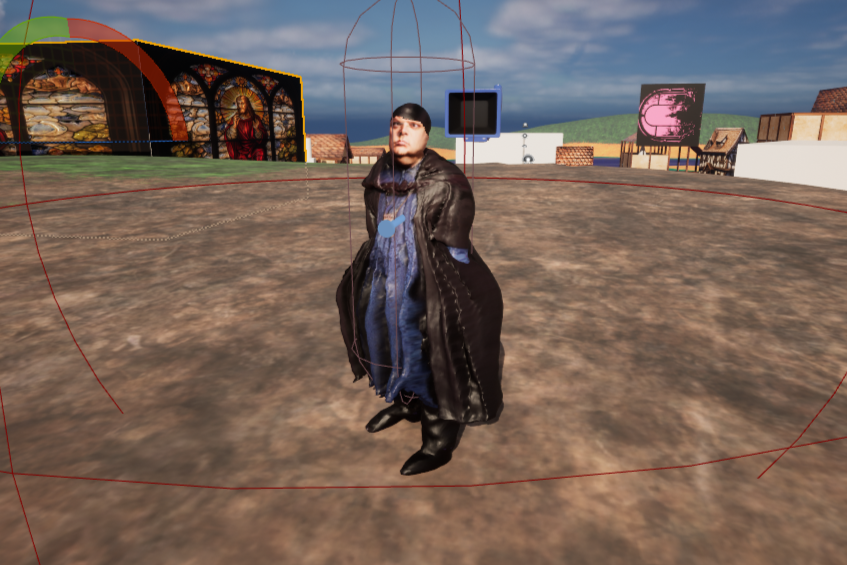
\includegraphics[width=14cm]{BilderFuerBA/MartinLutherImSpiel.png}
	\caption{UE5: Martin Luther im Spiel}
	\label{MartinLutherImSpiel}
\end{figure}
\\
Wie die genannten KI-Systeme verwendet werden, werde ich in den folgenden Absätzen erklären.
\begin{figure}[h]
	\centering
	
\includegraphics[width=14cm]{BilderFuerBA/02.png}
	\caption{ChatGPT: Erster Versuch zur erstellung eines Promt für Midjourney}
	\label{ChatGPT_erster_Versuch_Midjourney_Promt}
\end{figure}
\begin{figure}
	\centering
	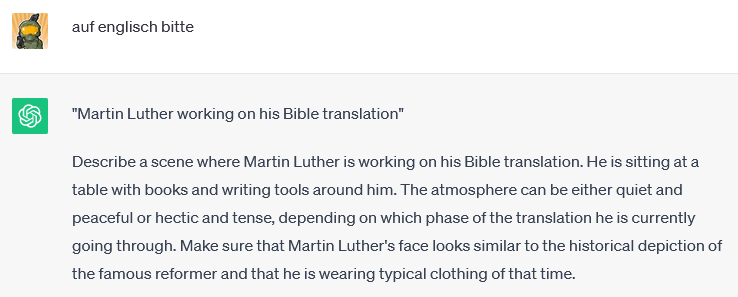
\includegraphics[width=14cm]{BilderFuerBA/03.png}
	\caption{ChatGPT: Übersetzung des Prompts}
	\label{ChatGPT_übersetzen}
\end{figure}
\\
Ich beginne die Entwicklung der Hauptfigur in dem ich ChatGPT um eine Beschreibung meiner Hauptfigur auffordere. Ich gebe ebenfalls an, dass ich die Ausgabe von ChatGPT als Prompt für Midjourney verwenden möchte. Zusätzlich fordere ich ChatGPT auf, dass das Ergebnis von Midjourney für PIFuHD kompatibel sein soll.
\\
Mit der in Abbildung \ref{ChatGPT_erster_Versuch_Midjourney_Promt} zusehenden Aufforderung, habe ich eine deutsche Ausgabe bekommen. 



Durch eine weitere kurze Aufforderung wie in Abbildung \ref{ChatGPT_übersetzen} wird die Ausgabe von ChatGPT ins Englische übersetzt.
\begin{comment}
	\begin{figure}
		\centering
		\begin{minipage}[t]{0.45\linewidth}
			\centering
			\includegraphics[width=6.405cm]{BilderFuerBA/Busfahrer.png}
			\caption{Midjourney Prompt: Bussfahrer}
			\label{Bussfahrer}
		\end{minipage}
		\hfill
		\begin{minipage}[t]{0.45\linewidth}
			\centering
			\includegraphics[width=6.405cm]{BilderFuerBA/bus_driver.png}
			\caption{Midjourney Prompt: bus driver}
			\label{bus_driver}
		\end{minipage}
	\end{figure}
	\\
	Midjourney liefert in Englisch in Gegensatz im Vergleich zu Deutsch oft unterschiedliche Ergebnisse. Beobachten kann das zum Beispiel in Abbildung \ref{Bussfahrer} Bussfahrer auf deutsch, und in Abbildung \ref{bus_driver} buss driver auf englisch.
	\\
	Anhang in Abbildung \ref{Bussfahrer} und Abbildung \ref{bus_driver} kann man gut beobachten, dass die verwendeten Sprache einen Unterschied macht. Im Englischen wird eher eine Person dargestellt, die ein Lenkrad in der Hand hält, wo der Prompt auf deutsch eher ein Passagier dargestellt wird oder ein Bus in einer Landschaft.
\end{comment}
\\
%https://philipp-stelzel.com/de/midjourney-deutsch-sprachen/ Abrufdatum 25.09.2023
Midjourney versteht nicht unsere Sprache, sondert die Genauigkeit entsteht aus der Menge der Daten womit das KI-System Trainiert ist. Das Wort Bussfahrer kommt womöglich nicht so oft in den Trainigsdaten vor wie buss driver aus dem Englischen.
\\
Mit dieser Erkenntnis, entscheide ich mich meine Promts auf Englisch für Midjourney zu verfassen beziehungsweise von ChatGPT verfassen lassen.
\begin{figure}[h]
	\centering
	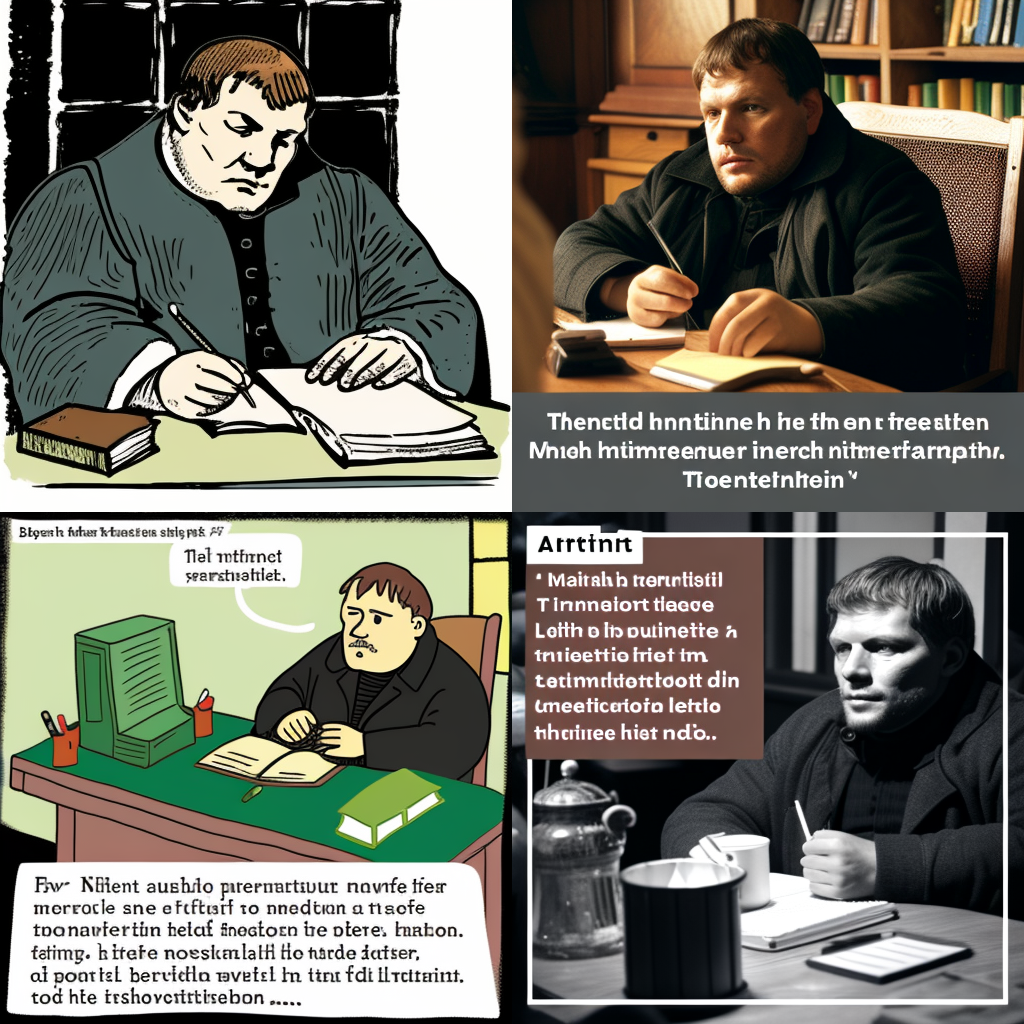
\includegraphics[width=8.022cm]{BilderFuerBA/MLaufEnglisch.png}
	\caption{Midjourney: Erster Prompt von ChatCPT}
	\label{Midjourney_erster_Prompt}
\end{figure}
\\
Nach der Übersetzung von ChatGPT, übergebe ich den von ChatGPT generierten Midjourney-Promt Midjourney. Das erste Ergebnis mit dem von ChatGPT generierten Midjourney-Prompt aus \ref{ChatGPT_übersetzen} is in Abbildung \ref{Midjourney_erster_Prompt} zu betrachen.
\\
Der Midjourney-Prompt von ChatGPT aus Abbildung \ref{ChatGPT_übersetzen} beinhaltet sehr viele Schlüsselwörter und ist sehr Athomsphärisch geschreiben, wie als würde es aus einer Textstelle von einem Roman kommen, anstelle einer Aufforderung gegenüber eines KI-Systems.
\begin{figure}[h]
	\centering
	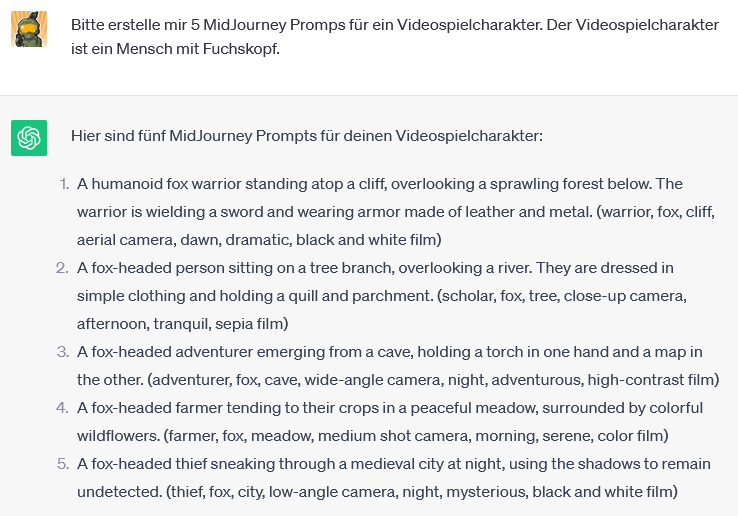
\includegraphics[width=14cm]{BilderFuerBA/05.png}
	\caption{ChatGPT: Erstellung Prompts mit Verwendung der Midjourney-Formel}
	\label{chatgpt_mj-formel_mit_Klammern}
\end{figure}
\begin{figure}[h]
	\centering
	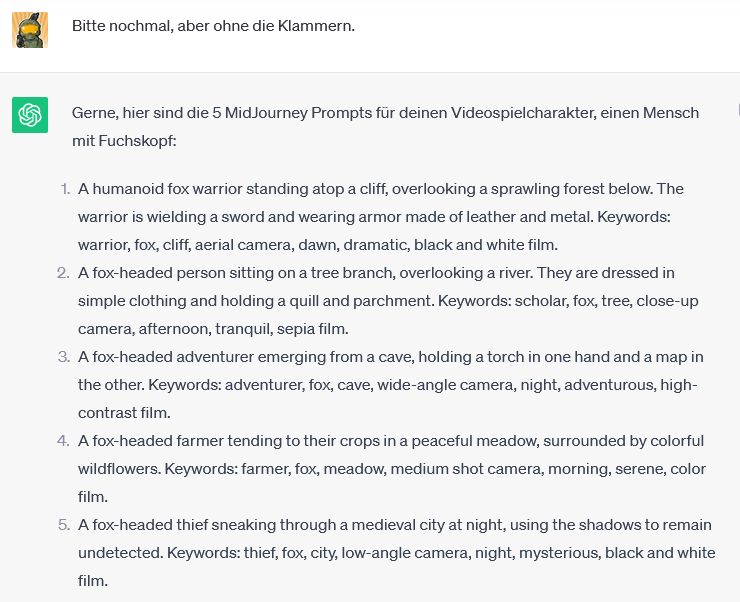
\includegraphics[scale=0.7]{BilderFuerBA/06.png}
	\caption{ChatGPT: ChatGPT erstellt Promt für Midjourney in Englisch und ohne Klammern}
	\label{chatgpt_mj-formel_ohne_Klammern}
\end{figure}
%Ich vermutet, dass ChatGPT nicht genügend darauf trainiert ist, wie Midjourney-Prompts auszusehen haben.
%\\
\begin{figure}[h]
	\centering
	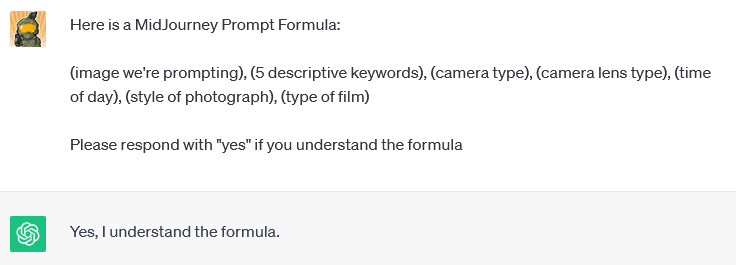
\includegraphics[width=14cm]{BilderFuerBA/04.png}
	\caption{ChatGPT: Aufforderung verwendung einer Midjourney-Formel}
	\label{chatgpt-ptompt-Midjourney-04}
\end{figure}
\\
Eine Recherche auf YouTube hat zeigt, dass das Verwenden von Midjourney-Formeln ein aufgeräumtes Ergebnis hervorbringen kann. Eine Kurze Auforderung wie in Abbildung \ref{chatgpt-ptompt-Midjourney-04} kann bessere Ergebnisse bei Midjourney gewähren.
\\
Im ersten Test werden die Prompts mit Klammern \ref{chatgpt_mj-formel_mit_Klammern} ausgegeben. Diese sind mit einer einfachen Aufforderung wie in \ref{chatgpt_mj-formel_ohne_Klammern} möglich zu entfernen.
\\
\begin{figure}
	\centering
	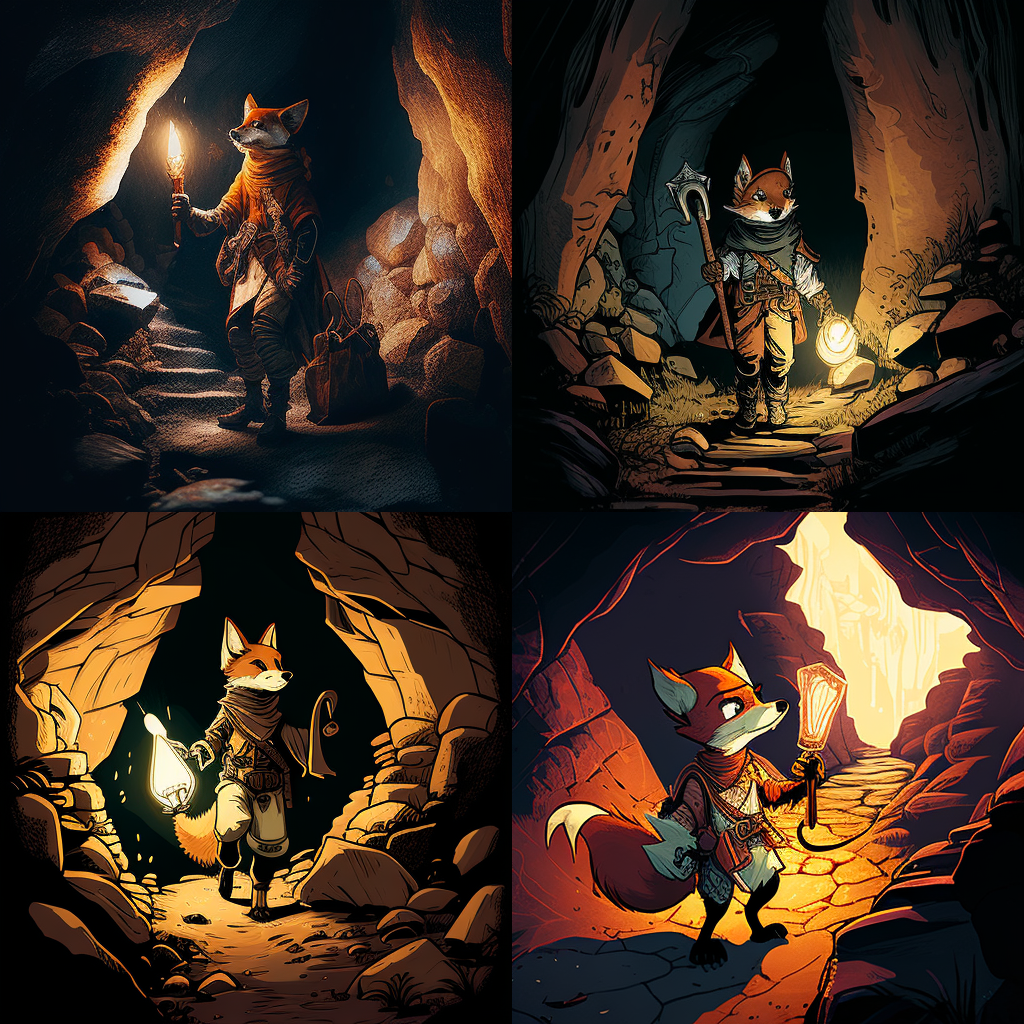
\includegraphics[width=8.022cm]{BilderFuerBA/fuchsKopfAbenteuerer.png}
	\caption{Midjourney: Promt eines Abenteurers mit einem Fuchskopf}
	\label{MidjourneyFuchsKopfAbenteuerer}
\end{figure}
\\
Ich habe die Ausgabe von ChatGPT über einen Abenteuerer mit Fuchskopf als Prompt an Midjourney übergeben und das Ergebnis ist in Abbildung \ref{MidjourneyFuchsKopfAbenteuerer} zu sehen.
\\
\begin{figure}
	\centering
	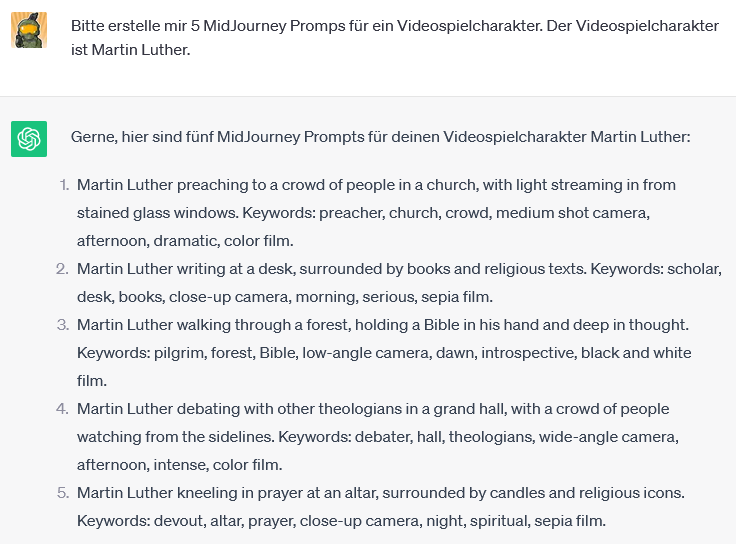
\includegraphics[scale=0.7]{BilderFuerBA/07.png}
	\caption{ChatGPT: Midjourney Prompt für Martin Luther als Spielfigur}
	\label{chatgptMartinLutherMJformelErstenFünf}
\end{figure}
\\
Da mein Hauptcharakter kein Abenteurer mit Fuchskopf ist, sonder Martin Luther nachempfunden sein soll, habe ich ChatGPT dazu Aufgefordert mir 5 Promts für Midjourney zu erstellen um Bilder von Martin Luther generieren zu lassen. Die Ergebnisse von ChatGPT ist in Abbildung \ref{chatgptMartinLutherMJformelErstenFünf} zu betrachten. Abbildung \ref{MidJourneyMLMitFormel} zeigt die daruas von Midjourney generierten Bilder.
\begin{figure}
	\centering
	
\includegraphics[width=8.022cm]{BilderFuerBA/MidJourneyMLMitFormel.png}
	\caption{Midjourney: Martin Luther Promt mit Midjourney-Formel}
	\label{MidJourneyMLMitFormel}
\end{figure}
\\
An dieser Stelle haben ich ChatGPT soweit gebracht, dass ChatGPT mir strukutierte Midjourney-Promts generiert. Das nächste Ziel ist, das nicht nur die Midjourney-Prompts stukturiert sind, sondern auch die daraus resultierenden Bilder, die später mit Hilfe von PIFuHD 3D-Modelle erzugt. Bilder wie die aus Abbildung  \ref{MidJourneyMLMitFormel} sind noch nicht geeignet um gute Ergebnisse von PIFuHD zu bekommen. Dieses Ergenis ist zum Beispiel farbenfroh und beinhaltet viele Deteils im Hintergrund was zu einem nicht guten Ergibnis führen würde.
\\
Hier eine Aufzählung mit Eigenschaften von Bilder, die PIFuHD benötigt um gut zu Arbeiten:
\\
Die zu verwendeten Bilder sollten:
\begin{itemize}
	\item eine Mindestauflösung von 512 x 512 Pixel haben.
	\item nur eine Person zeigt und direkt in die Kamera schaut.
	\item eine gut beleuchtet Person zeigen.
	\item einen einfachen Hintergrund besitzen.
\end{itemize}
\begin{figure}
	\centering
	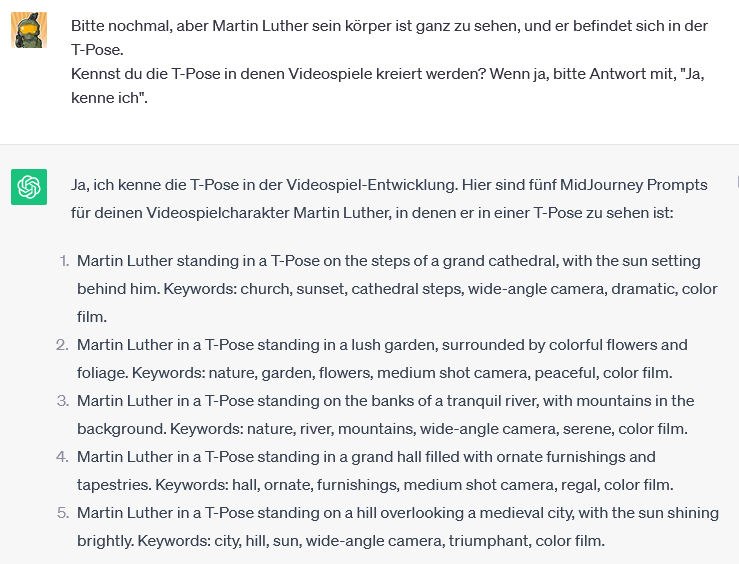
\includegraphics[scale=0.7]{BilderFuerBA/09.png}
	\caption{ChatGPT: Midjourney Prompt für Martin Luther in T-Pose}
	\label{chatgptMartinLutherMJinTPose}
\end{figure}
Um diese Punkte zu beachten habe ich folgende Parameter von ChatGPT überarbeiten lassen. Als erstes soll der Charakter in der T-Poste stellung sein Abbildung \ref{chatgptMartinLutherMJinTPose} anschließend mit einem Neutralen Hintergrund und einer direkten Kamere auf die Figur. Das Ergebnis ist in Abbildung \ref{MartinLutherInTPoseNeutralerHintergrundDirekteKamera} zu sehen.
\\
An dieser Stelle habe ich nicht mehr mit ChatGPT für die Hauptfigur gearbeitet. Ab hier habe ich sehr viel ausprobiert um eine Fotoähnliche abbildung von Martin Luther zu bekommen. Der Finale Prompt der am ende das Bild von Martin Luther generiert hat war:
\\
\rmfamily
\begin{large}
	the famous martin luther from germany, robe from the Renaissance, T-Pose for gamedesign, standing in front of a plain blue background. neutral magenta background, T-Pose, whole body, face looking in the camera, color film
\end{large}
\sffamily
%\\
%Midjourney
\\
Mit diesem Prompt habe ich es geschafft in Abbildung \ref{ErsteAusgabeVomFinalenPrompt} ein Ergebnis zu generieren was meine Anforderung als Ein-Mann-Vidospielentwickler entspricht. Ich habe ein, gerade in die Kamera schauende Mann der Martin Luther ähnlich sieht. Der Mann steht in einer T-Pose. Der Hintergrund ist farbarm / neutral und der komplette Körper ist zu sehen. 
\\
%todo user-Interface erklären
In Abbildung \ref{ErsteAusgabeVomFinalenPrompt} ist zu sehen, das Midjourney immer Vier Bilder als Vorschau ausgibt. Midjourney bietet über sein User-Interface drei Möglichkeiten um mit dem Ergebnis weiter zu Arbeiten:
\begin{itemize}
	\item 1 Vier weitere Versionen auf grundlage von Version 1 bis 4 über Button V1 bis V4
	\item 2 Eine Hochskallierte Version von 1 bis 4 über die Button U1 bis U4
	\item 3 Vier neue weitere Versionen über den kreisrudnen Pfeilbutton
\end{itemize}
Oben links befindet sich Version 1, oben rechts Version 2, unten links Version 3 und unten rechts Verion 4.
\\
Durch die betätigung des Buttons V2 bekomme ich 4 weiter Versionen auf grundlage von Version 2 aus der Abbildung \ref{ErsteAusgabeVomFinalenPrompt}.
\begin{figure}
	\centering
	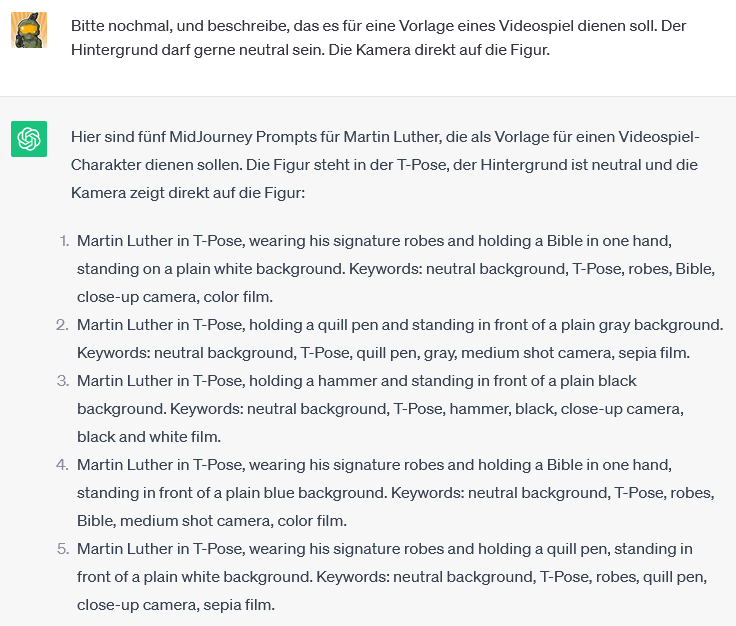
\includegraphics[scale=0.7]{BilderFuerBA/10.png}
	\caption{ChatGPT: Midjourney Prompt für Martin Luther in T-Pose}
	\label{chatgptMartinLutherMJmitNeutralenHintergrund}
\end{figure}
\begin{figure}
	\centering
	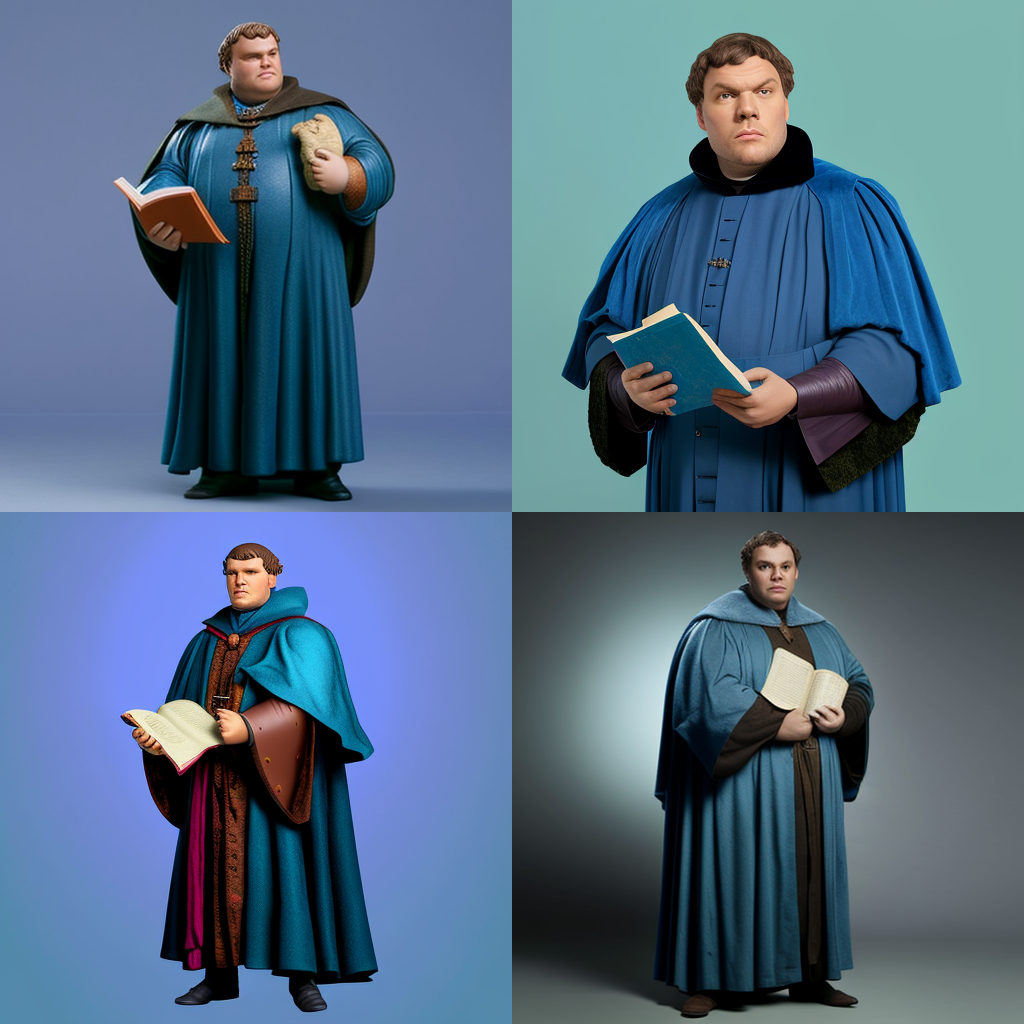
\includegraphics[width=8.022cm]{BilderFuerBA/MartinLutherInTPoseFirst.png}
	\caption{Midjourney: Martin Luther Promt versuch in T-Pose, neutralen Hintergrund und direkte Kamera}
	\label{MartinLutherInTPoseNeutralerHintergrundDirekteKamera}
\end{figure}
\begin{figure}
	\centering
	\includegraphics[width=8.022cm]{BilderFuerBA/ErsteAusgabeVomFinalenPrompt.png}
	\caption{Midjourney: Erste Ausgabe vom finalen Prompt}
	\label{ErsteAusgabeVomFinalenPrompt}
\end{figure}
\begin{figure}
	\centering
	\includegraphics[width=8.022cm]{BilderFuerBA/ZweiteAusgabeVomFinalenPrompt.png}
	\caption{Midjourney: Vier weitere Variation von Version Zwei}
	\label{ZweiteAusgabeVomFinalenPrompt}
\end{figure}
\\
Abbildung \ref{ZweiteAusgabeVomFinalenPrompt} zeigt vier weitere Versionen von Version 2 der Ausgabe \ref{ErsteAusgabeVomFinalenPrompt}. Die Unterschiede sind viel geringer und unterscheiden sich in diesem Beispiel am größten an der Frisur, den Oberteil der Robe und der Kette.
\\
Die Kette in Version 4 ist ein Deteil die ich an meinem Hauptcharakter sehen möchte und somit entscheide ich mich dafür, Version Vier über den Button U4 hochzuskaliern.
\begin{figure}
	\centering
	
\includegraphics[width=8.022cm]{BilderFuerBA/DritteAusgabeVomFinalenPrompt.png}
	\caption{Midjourney: Hochskaliertes Endresultat von Version Vier}
	\label{DritteAusgabeVomFinalenPrompt}
\end{figure}
\\
Die hochskalierte Version von Abbildung \ref{ZweiteAusgabeVomFinalenPrompt} ist in Abbildung \ref{DritteAusgabeVomFinalenPrompt} zu betrachten.
\\
Wir sehen einen Mann in einer Kirchlich anmutenden Robe. Sein Haar ist braun, seine Haut hell. Der Mann trägt beide Arme vom Körper so das die Handinnenfläche zur Kamera zeigen, was alle Kriterien für eine Verwendung mit PIFuHD besitzt, bis auf die Tatsache, das dieses Foto kein echtes Foto ist, sonder durch ein KI-System generiertes Bild ist.
\\
Dieses Bild von Martin Luther verwende ich den Folgenden Kapitel als Vorlage für PIFuHD, um ein 3D-Modell von Martin Luther zu bekommen.
\subsection{Erzeugen eines 3D-Modells mit Hilfe von PIFuHD}
\begin{figure}
	\centering
	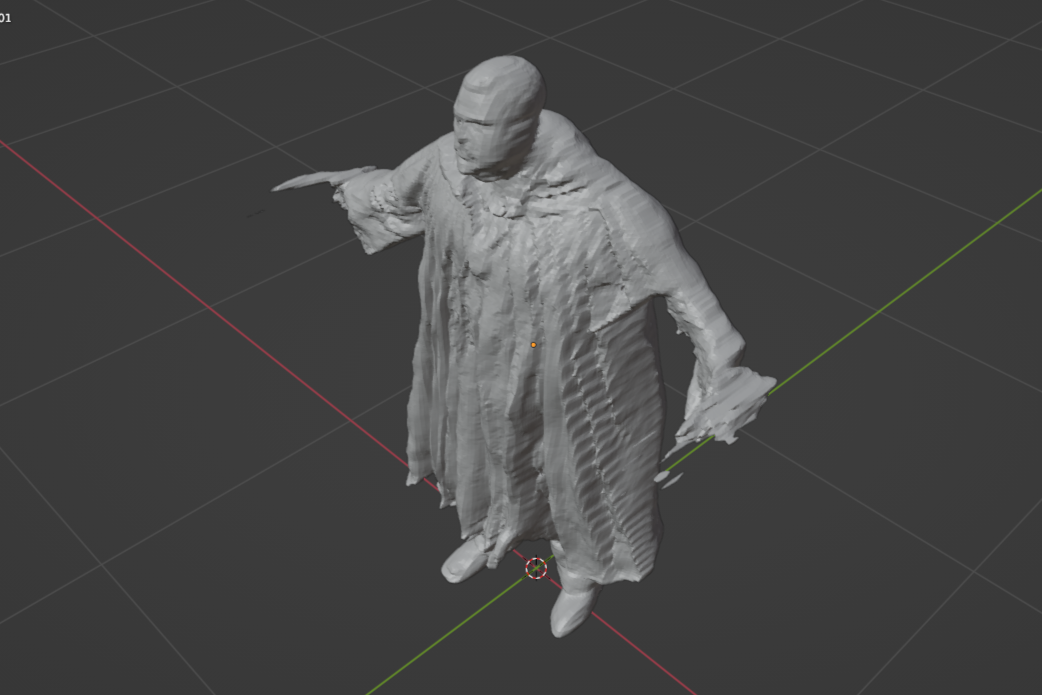
\includegraphics[width=14cm]{BilderFuerBA/BlenderMLVonPIFuHD105k.png}
	\caption{Blender: 3D-Modell von Martin Luther von PIFuHD}
	\label{BlenderMLVonPIFuHD105k}
\end{figure}
\begin{figure}
	\centering
	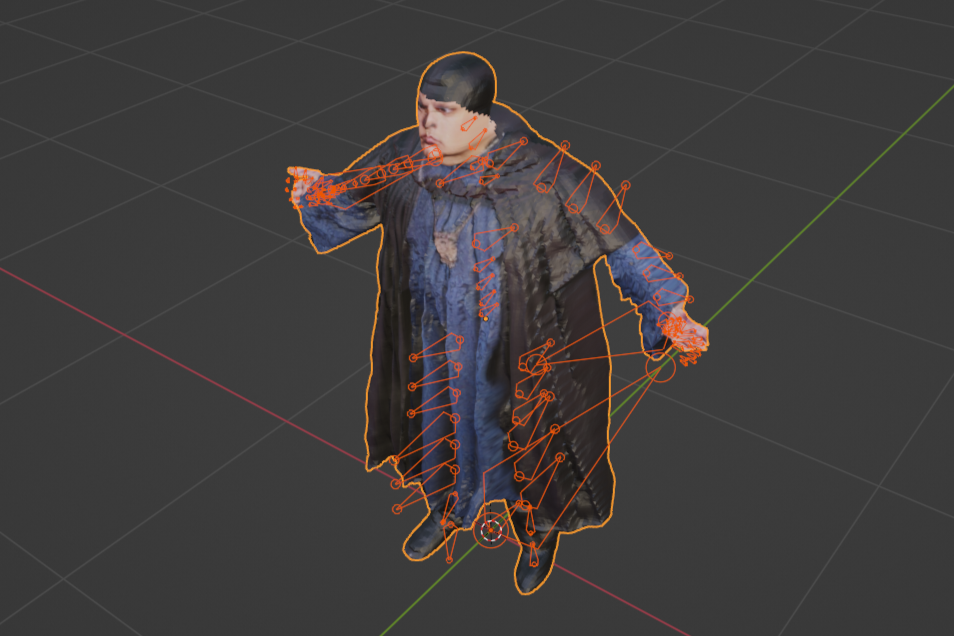
\includegraphics[width=14cm]{BilderFuerBA/BlenderMLGeriggtUndTexturiert95k.png}
	\caption{Blender: Martin Luther Texturiert, geriggt, Nachgebessert und gemergeten Verticies}
	\label{BlenderMLGeriggtUndTexturiert95k}
\end{figure}
In Abbildung \ref{BlenderMLVonPIFuHD105k} zeigt das 3D-Modell von Martin Luther welches durch das KI-System PIFuHD erzeugt ist.
\\
PIFuHD ist durch eine Google-Suche zu finden. Der Erste Vorschlag von Google zeigt eine Git-Hub-Link an. Im kopf dieser Git-Hub Seite findet man weit oben den Link zur Demo die auf Google-Colab veröffentlicht ist.
\\
Über das Anmelden meins Google-Kontos und über das Verbinden mit der gehosteten Laufzeig bringe ich über Google-Colab die Demo von PIFuHD zum Laufen.
\begin{comment}
	Ich habe die Demo über Google-Colab zum laufen bekommen in dem ich mich über mein Google-Konto anmelde und auf Verbinden mit gehosteter Laufzeit: GPU klicke.
\end{comment}
\\
Anschließend starte ich über den Menüpunkt Laufzeit → Alle ausführen oder alternativ CTRL + F9 PIFuHD.
\\
Weiter unten in der Website befindet sich der Abschnitt Config input data. An dieser Stelle wartet PIFuHD auf meine Eingabeauforderung, wo ich mein Bild Abbildung \ref{DritteAusgabeVomFinalenPrompt} übergebe.
\\
Die Übergabe folgt über den Button Durchsuchen.... Ist die Übergabe erfolgreich, erfolgt die Ausgabe über der Ordnerstruktur links.
\\
Meine obj-Datei befindet sich unter pifuhd → results → pifuhd-final → recon. Zusätlich zu meiner obj-Datei bietet PIFuHD mir eine png-Datei an, was eine Normalmap darstell und eine mp4-datei die ein fünf sekündiges Video von meinem 3D-Modell zeigt.
\\
%todo Polycount, UVs und narnite erklären verionsnummern hinzufügen
\begin{comment}
	Das 3DModell beinhaltet Verticies auserhalb des 3D-Modells von Martin Luther. Diese Verticies lösche ich in dem ich alle Verticies in dem ich den Shortcut A drücke. Anschließend Unwrape ich mein 3D-Modell in dem ich den Shortcut U drücke.
\end{comment}
\begin{comment}
	Der Vorteil dieser Methode ist, das man nun einzelne Parameter in der Midjourney-Formel belieben verändern kann um ein Gewünschtes Ergebnis zu erlangen. Das Ziel ist es ein "Foto" von Martin Luther zu bekommen um es später für PIFuHD zu verwenden. Das Ergebnis von Abbildung \ref{MidJourneyMLMitFormel} ist noch nicht zu verwenden, da zu viele Fabenfrohe Deteils zu sehen sind. PIFuHD weist darauf hin das Bilder am besten funktionieren wenn die zu verwendeten Bilder:
\end{comment}
\subsection{Polycount verringern in Blender}
in Blender kann über den Menüpunkt File → Import → Wavefront die Obj-Datei importiert werden. 
\\
Das verringern des Polycount bewirkt, dass im späteren Prototyp weniger rechenkapazität verwendet wird.
\\
Nachdem ich die Obj-Datei in Blender Importiert habe, wechsel ich in den Eddit Mode.Im Edit Mode wähle ich ein Verticie mit der rechten Maustaste aus. Mit STRG + L wähle ich alle mit dem Modell verbundene Verticies aus. Das Modell erscheint nun Orange. Mit der Tastenkombination STRG + I invertiere ich die Auswahl. Nun habe ich alle Verticies ausgewählt die nicht direkt Mit dem 3D-Modell verbunden sind. Mit der dem Shortcut X ist es mir nun möglich alle Verticies zu löschen die auserhalb des 3D-Modells liegen.
\\
Nach dem ich Alle Verticies die ausherhalb der 3D-Modells von Martin Luther gelöscht wurden, werde ich den Polycount von der Hauptfigur verringern. PIFuHD erzeugt Verticies die die gleichen oder sehr nahe Coordinaten besitzen. Diese Verticies verwenden im Spiel unötig Rechenkapazität. Um Verticies die zu nach zueinander zu löchen stellt Blender Die Funktion Merge zu verfügung.
\\
Damit ich Alle Verticies des 3D-Modells Merge wähle ich erneut alle Verticies mit dem Shortcut A aus. Da nun alle Verticies ausgewählt sind, ist er mir nun möglich mit dem Shortcut M das 3D-Modell zu mergen. Nach der betätigung des Shorcuts M wähle ich die Merge-Funktion By Distance. Ich ändere unten links üder das kleine Untermenü, die den Namen Merge by Distance trägt, den wert von 0,0001~m auf 0,001~m.
\\
Nun sind alle Verticies die eine geringere Distance als 1 mm voneinander entfernt sind gelöscht und neu verbunden und der Polywert wurde von knapp 120.000 Verticies auf 98.000 Verticies verringert, was eine Verringerung von rund 18\% ist.
\\
\subsection{Artefakte bereinigen in Blender}%todo artefakt Artefakte bezeichnet man zu dt.: auch als Bildfehler oder Darstellungsfehler bei Video oder Bilddateien. Sie entstehen durch Fehlberechnungen, Übertragungsfehler oder durch eine zu hohe Kompressionsrate beim Komprimieren der Bild- oder Videodateien. Artefakte zeigen sich in den meisten Fällen als Klötzchen im Bild. https://www.caseking.de/glossar/a/artefakt
PIFuHD Arbeitet nicht perfekt und erzeugt grob sichtbare Fehler. Besonder die Bereiche an den Händen und Füßen ist es immerwieder zu sehen, das sie mangelhaft erstellt werden. In Blender gibt eine vielzahl an Möglichkeiten sein 3D-Modell zu bearbeiten. Ich habe nachdem ich den Polycount reduziert habe betreffende Stellen im Edit Mode makiert und mit einer größeren Distance gemerget. Ein weiteres Verfahren war im Sculp Mode die verschiedenen Sculpwerkzeuge zu verwenden wie zum Beispiel Draw um die betroffenen stellen zu bearbeiten.
\subsection{Texturieren in Blender}
\begin{comment}
	zweites bearbeitungsfenster hinzufügen auf UV-Editor umstellen über menüpunkt Image - Open das gewünschte foto... die kamera so einstellen das es ungefähr die gleiche blickrichtung auf das model hat wie im bild... in dem beispiel kann man über das numbap 1 für frontalansich wählen..
	im modell alles makieren und mit dem shortkut u für unwrap die funktion Projekt from View auswählen.
	Skallieren im UV Editor
\end{comment}
Damit ich in meinen Prototyp keine graue Figur zum spielen habe, benötigt die Hauptfigur eine Textur. Diese Textur stammt von Abbildung \ref{DritteAusgabeVomFinalenPrompt}, was els Eingabematerial verwendet wurde um mit PIFuHD ein 3D-Modell zu erzeugen. Kurz, in diesem Abschnit erkläre ich, wie ich das Eingabebild und das 3D-Modell von PIFuHD miteinander Verbinde.
\\
Blender bietet mir die Möglichkeit ein zweites Bearbeitungsfenster hinzuzufügen, welche ich dann als UV Editor benutze. Über den Menüpunkt Image → Open, füge ich Abbildung \ref{DritteAusgabeVomFinalenPrompt} ein, um UVs des 3D-Modells zu bearbeiten. Rechts über das Propertie-Fenster → Material Properties → der gelben Punkt neben Base Color → Image Textur, habe ich nun die Möglichkeit, ebenfalls Das Bild aus Abbildung \ref{DritteAusgabeVomFinalenPrompt} zu wählen, welche die Standartmaterialeigenschaft in eine Image Textur umwandelt.
\\
Damit das Bild von Martin Luther korrekt auf das 3D-Modell von Martin Luther projeziert wird, wähle ich eine Kameraeinstellung, die ungefähr der Kameraeinstellung aus \ref{DritteAusgabeVomFinalenPrompt} entsprich. Ma mein Bild von Martin Luther eine Direkte von vorne gerichtete Fotografie zeikt, wird durch die Betätigung der 1 auf meinem Numpad die Kamera so eingestellt das ich eine frontale ansicht meines 3D-Modells im Edit Modus bekomme.
\\
Ich Makiere alle Verticies in dem ich den Shortcut A drücke. Anschließend Unwrape ich mein 3D-Modell in dem ich den Shortcut U drücke. Blender bietet mir verschiedene Fuktionen an, mein 3D-Modell zu unwrapen. Ich wähle die Fuktion Project from View. In meinem UV-Editor habe ich nun die Möglichkeit, das Projezierte 3D-Modell so zu skalieren das es mit der Vorlage übereinstimmt.
\\
Das Problem nach dem Unwrapen, nach dieser beschriebenen Methode ist, dass das 3D-Modell von Vorne genauso texturiert ist wie von Hinten. Um den Rücken und den Hinterkopf einigermaßen korrekt zu texturieren, wähle ich die die ensprechenden Bereiche aus und verschiebe sie im UV-Editor in Bereichen, die zu dieser Stelle die im Bild eher passen würden.
\\
Zum Beispiel der Mittelteil der Robe, der blau gefärbt ist, verschiebe ich in eine etwas brauneren Region im UV-Editor.
\\
Nachdem ich den Rücken und den Kopf nachtexturiert habe, fehlt noch ein letzer wichtiger schritt, damit Martin Luther in der Unreal Engine zum Leben erweckt wird, und zwar das Rigging.


\subsection{Rigging in Blender}%todo rigging erklären
Damit mein Hauptcharakter nicht nur in seiner T-Pose verweilt wenn er läuft und Springt, sonder Arme Beine und Kopf bewegt, braucht das 3D-Modell von Martin Luther ein Skeleton-Mesh.
\\
Bevor ich das 3D-Modell in Blender rigge, benötige ich das Blander Addon Game Rig Tools von CGDive.
\\
Über den Button Initiate Mannequin fügt das Addon ein Unreal Engine 5 kompatibles Skeleton Mesh zu mein 3D-Modell.Über das UE5\_Manny\_TWEAK das ich über die Scene Collection auswählen kann, bewege ich die einzelnen Bones des Skeleton-Mesh innerhalb des 3D-Modells. Mit dem Shortcut G kann ich im Pose Mode die einzelnen Bones bewegen.
\\
%toto verbindung zwichen rig und modell noch beschreiben
\\
Nachdem ich die Bones vom UE5\_Manny\_TWEAK fertig platziert habe, kann ich über das Addon-Fenster von Game Rig Tool, das Unreal-Rig nur sichtbar machen in den ich auf den Weißen Punkt neben Unreal drücke. 
\\
Nachdem nur noch unser 3D-Modell und das Unreal-Rig sichtbar ist wechsel ich in den Object Mode und wähle erst mein 3D-Modell aus und mit Schift-Taste gedrückt das Unreal-Rig.
\\
Da ich nun Das 3D-Modell von Martin Luther und das Unreal-Rig im Objekt Mode in der korrekten Reihenfolge ausgewählt habe, kann ich nun über den Menüpunkt File → Export → FBX, das geriggte Modell speichern. Beim Speichern wähle ich folgende Optionen aus:
\begin{itemize}
	\item Limit to Selected Objects 
	\item Object Types; Amature und Mesh
	\item Unter Transform bestätige ich das Apply Transform
	\item Unter Geometry wähle ich unter Smoothing → Face
	\item Unter Armature stelle ich Add Leaf Bones aus
	\item Bake Animation stelle ich ebenfalls aus
\end{itemize}
Nachdem ich diese Einstellung getätigt habe, wähle ich noch ein Namen für meine FBX-Datei und drücke auf Export FBX.

\subsection{Einfügen des Haupcharakters in Unreal Engine 5}
Der Haupcharakter ist soweit fertig zum Importieren in die Unreal Engine 5, danach kann ich mich mit ihm in der Unreal Engine 5 testen.
\\
Über den Epic Games Launcher erstelle ich ein neues Projekt. Ich benutze das Third-Person-Template was mir eine kleine Arena und ein Videospielcharakter vorgibt. Ich benutze die Project Default-Einstellung Blueprint. Zum Schluss gebe ich mein Projekt noch einen Namen und erstelle Mein Projekt mit Create.
\\
In der Entwicklungsumgebung Unreal Engine 5 angekommen, suche ich nach der BP\_ThirdPersonCharacter Blueprint Class.
\\
Die BP\_ThirdPersonCharacter Blueprint Class befindet sich unter dem Ordner All → Content → ThirdPerson → Blueprints. Über den Button Import der sich im Contentbrowser befindet, kann ich meine durch Blender exportierte FBX-Datei importieren. Nach dem auswählen meiner FBX-Datei, öffnet sich die FBX-Importoptionnen, wo ich das SK\_Mannequin für das Skeleton auswähle. Anschließend klicke ich auf Import All.
\\
Um das Skeletal Mesh zu ersetzen doppelklicke ich auf das BP\_ThirdPersonCharacter Blueprint Class. Die BP\_ThirdPersonCharacter Blueprint Class besteht aus verschiedenen Components, von diesen verschiedenen Componets wähl ich das Mesh(CharacterMesh0) aus. Nach dem ich das Mesh(CharacterMesh0) ausgewählt habe, kann ich in den dazu geöffneten Details das Skeletal Mesh Asset durch mein Martin Luther tauschen. Automatisch wird auch die dazu gehörige Textur geändert.
\\
Nach diesen Schritten kann ich nun Martin Luther in meinem Prototyp als Hauptcharakter benutzen, in dem ich auf das grüne Play-Symbol klicke. Da ich mein 3D-Modell von Martin Luther mit BP\_ThirdPersonCharacter Blueprint Class verbunden habe, kann Martin Luther im spiel laufen und springen.
\begin{comment}
	\\
	Nun kann ich mit meinem Haupcharakter durch die vordefinierte ThirdPersonMap bewegen und springen. Ich habe sogar eine Kollision, was mich daran hindert durch den Boden und Wände zu laufen. Ich kann sogar gegen blaue Wüfel laufen, die physikalisch von mir beeinflusst werden.
\end{comment}
%
%
%
%
%
%
%
%\\\\\\\\\\\\\\\\\\\\\\\\\\\\\\\\\\\\\\\\\\\\\\\\\\\\ Gebäude\\\\\\\\\\\\\\\\\\\\\\\
%\\\\\\\\\\\\\\\\\\\\\\\\\\\\\\\\\\\\\\\\\\\\\\\\\\\\ Gebäude\\\\\\\\\\\\\\\\\\\\\\\
%\\\\\\\\\\\\\\\\\\\\\\\\\\\\\\\\\\\\\\\\\\\\\\\\\\\\ Gebäude\\\\\\\\\\\\\\\\\\\\\\\
\section{Meilenstein: Gebäude}
\begin{figure}
	\centering
	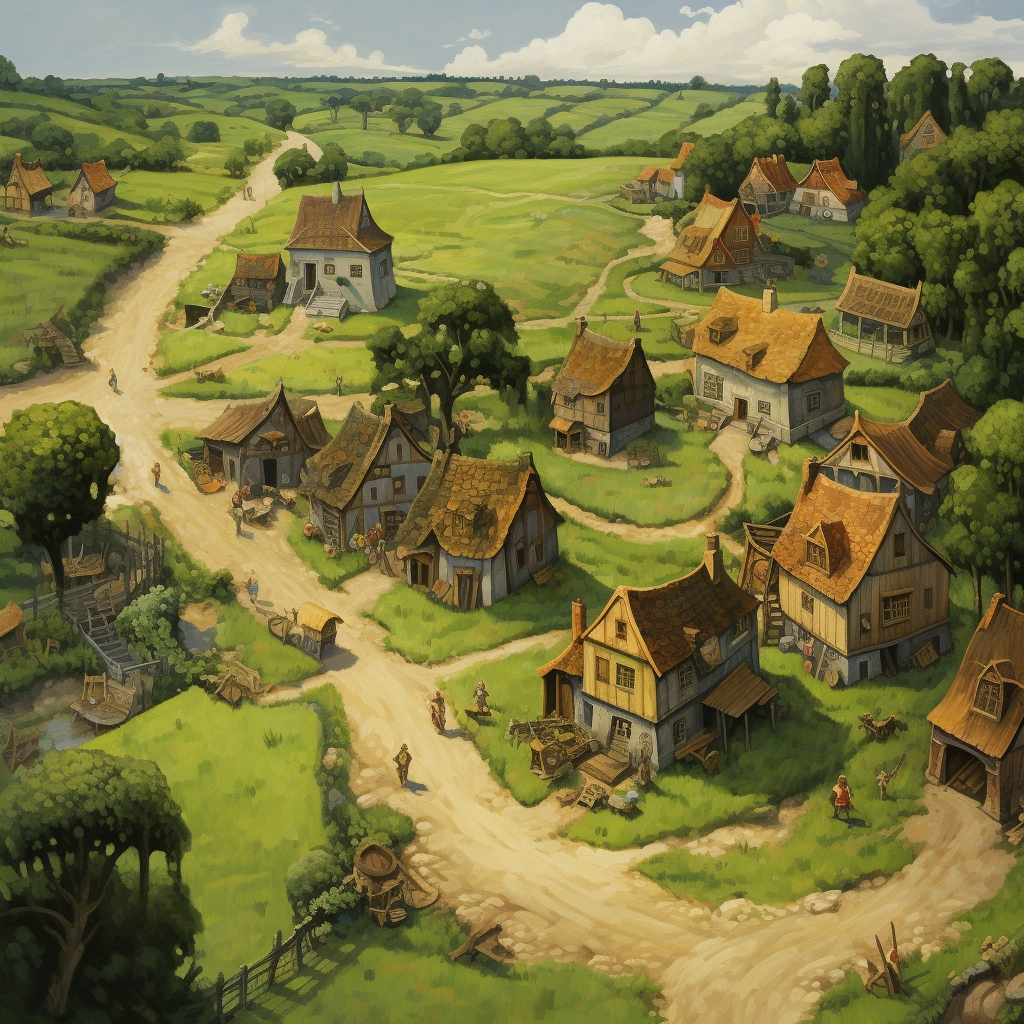
\includegraphics[scale=0.2]{BilderFuerBA/a_scatch_from_a_village_top_down.png}
	\caption{a scatch from a village, top down}
	\label{fig:Midjourney-Conceptart-Dorf}
\end{figure}
Nach der Erstellung der Hauptspielfigur, ist der nächste Schritt die Erstellung einer Spielwelt.
\\
Die Idee ist, ein Dorf in der Unreal Engine 5 zu erschaffen. In diesem Dorf befinden sich verschiedene Gebäude.
\\
In diesem Kapitel möchte ich zeigen, wie ich die Gebäude mit Hilfe verschiedener KI-Systeme in der Unreal Engine 5 realisiert habe. Ich werde in diesem Kapitel und in den folgenden Meilensteine nicht mehr detailliert auf alles wie bei der Erstellung der Hauptfigur eingehen, sondern nur auf Schritte, die sich im Prozess stark unterscheiden.
\\
Fachwerkhäuser repräsentieren etwas Mittelalterliches, und da die Renaissance zeitlich nach dem Mittelalter gegliedert ist, waren in Zeiten der Renaissance Fachwerkhäuser sehr weit verbreitet.
\\
Deshalb möchte ich diverse Fachwerkhäuser erschaffen und auf einer Landschaft verteilen, um eine Dorflandschaft zu erzeugen.
\\
\subsection{Erste Ansatz Fachwerkhäuser}%todo promts für die textur raussuchen
Mein erster Ansatz ist es, Häuser mit Hilfe von einem einfachen 3D-Modell umzusetzen, was ich in Blender erstellt habe. Dieses 3D-Modell bestand aus einem Quader mit einer Spitze. Kurz, ein einfaches Haus.
\\
Mit Midjourney habe ich Texturen erstellt, die Fachwerkhäuser nachempfunden sind. Diese Texturen und das einfache Haus wurden mit Hilfe von Blender verbunden.
\\
Folgend wurden die einfachen Fachwerkhäuser in Unreal Engine 5 Importiert und verteilt.
\\
Die erste Ansatz lässt funktioniert und man kann die Häuser frei auf einer Landschaft verteilen.

\subsection{Moddelieren und texturieren Einfaches Haus mit Blender}
\begin{figure}
	\centering
	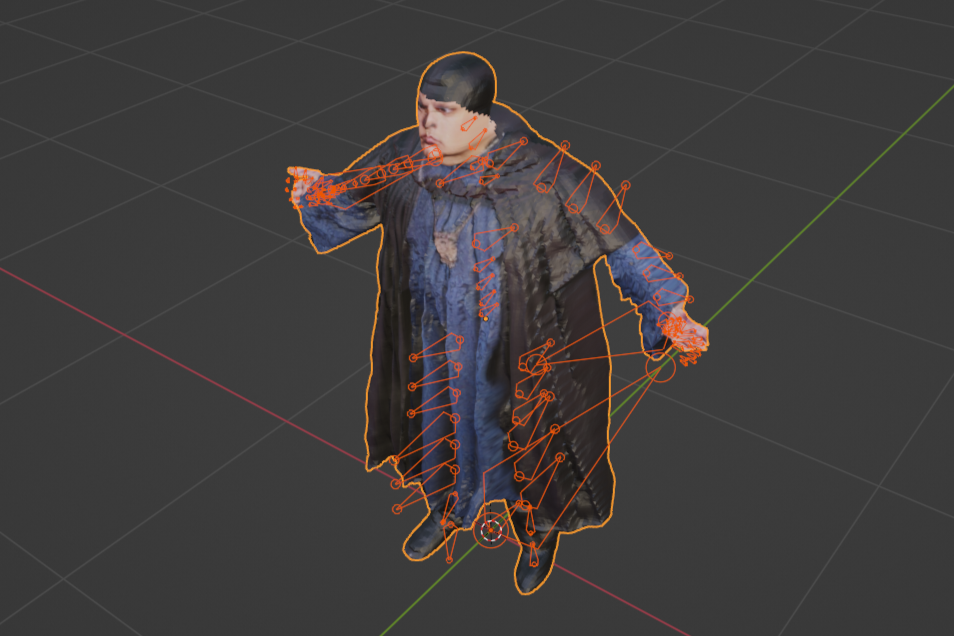
\includegraphics[width=14cm]{BilderFuerBA/BlenderMLGeriggtUndTexturiert95k.png}
	\caption{Blender: Martin Luther Texturiert, geriggt, Nachgebessert und gemergeten Verticies}
	\label{BlenderMLGeriggtUndTexturiert95k}
\end{figure}
Ich habe mit Blender eine einfache Würfel mit Spitze modelliert was mein einfaches Fachwerkhaus darstellen soll. Dieses Einfache Fachwerkhaus habe ich eine Textur übergeben die ich mit Midjourney erzuge.
\\
Beim Exportieren benötich ich keine Amature wie bei meiner Hauptfigur. Nach dem Exportieren kann ich die FBX datei in Unreal Engine 5 importieren.

\subsection{Zweiter Ansatz: Moddelieren eines Fachwerkhaus mit Blender}
%127 Cubes und 33 Planes
Mein zweite Ansatz ist, mit Blender Individuelle Häuser zu gestalten. Ich habe mit Midjourney Bilder von Fachwekhäuser gestalten lassen und versuch diese in Blender nach zu moddelieren.
\\
Das Haus habe ich 127 Cubes und 33 Planes in Blender erstellt un in Position gebracht. Zu meinem Moddelierten Haus, was nur aus dem Gefache bestand habe ich mit Hilfe von Planes als wände hinzugefügt.
%Dieser Prozess hat mehrere Tage und Stunden gekostet, was mich zum Dritten Ansatz gebracht hat.

\subsection{Dritter Ansatz Dorfbaukasten}%todo quellenn für valheim raussuchen

Eine Inspiration für meinen dritten Ansatz ist Valheim, ein Survival-Spiel von den Coffee Stain Studios. In diesem Spiel gibt es ein Baukastensystem, in dem der Spieler sein eigenes Haus bauen kann.
\\
In Valheim kann der Spieler verschiedene Wände, Balken, Fußböden, Dächer und Materialarten auswählen, um damit seine Behausung zu gestalten.
\\
Hinzu kommen andere Elemente wie Zäune und Gemüse um ein Garten zu erschaffen, Werkbänke, Tische und Stühle um eine Inneneinrichtung zu kreieren und sogar Teppiche aus Tierfelle und Trophäen die man an die Wand hängen kann um eine Dekorative Charakter in die Behausung eines Spielers zu schaffen.
\\
Aus dieser Inspiration habe ich einen dritten Ansatz entwickelt und zwar einen so genannten Dorfbaukasten.
\\
Dieser Dorfbaukasten besteht ebenfalls aus Wänden, Balken, Dächer, Dachgiebel, Fußböden und Tapeten.
\\
Aus meiner Beobachtung als Ein-Mann-Videospielentwickler, besteht ein Fachwerkhaus nur aus simplen Geometrien, wie zum Beispiel aus verschiedene Quader für Wände, Balken, Dach, Türen und Fenster. Der Dachgiebel von einem Fachwerkhaus ist ein dreieckiges Prisma. Diese einzelnen Elemente möchte ich nachbauen, so dass man in der Unreal Engine 5 einen Baukasten aus verschiedenen Einzelelementen verfügt um damit seine Fachwerkhäuser zu bauen. 
\\
Ein weiteres Ziel ist, diese einzelnen Elemente zu programmieren, damit die Materialeigenschaft sich untereinander unterscheiden. Das hat den Zweck, das die Spielwelt nicht zu monoton wirkt.
\\
Ein beispiel ist der Balken den ich mit ein neuen Blueprint Class vom typ Actor erstelle. Ich öffne die Blueprint Class einem doppelklick und füge über ADD Componets ein Cube hinzufügen. Diesen Cube skaliere ich in der X- und Y-Achse auf 0,4 der aus dem Würfel einen ein Meter hohen Balken mit 40 cm breiten und tiefen Profil.
\\
Im Construction Script kann ich mit Hilfe von Nodes meinen Balken besondere Eigenschaften geben wie, zufällige Auswahl von Materialien oder das bestimmen der Länge mit Hilfe eines Parameters.
\\
\begin{figure}
	%\centering
	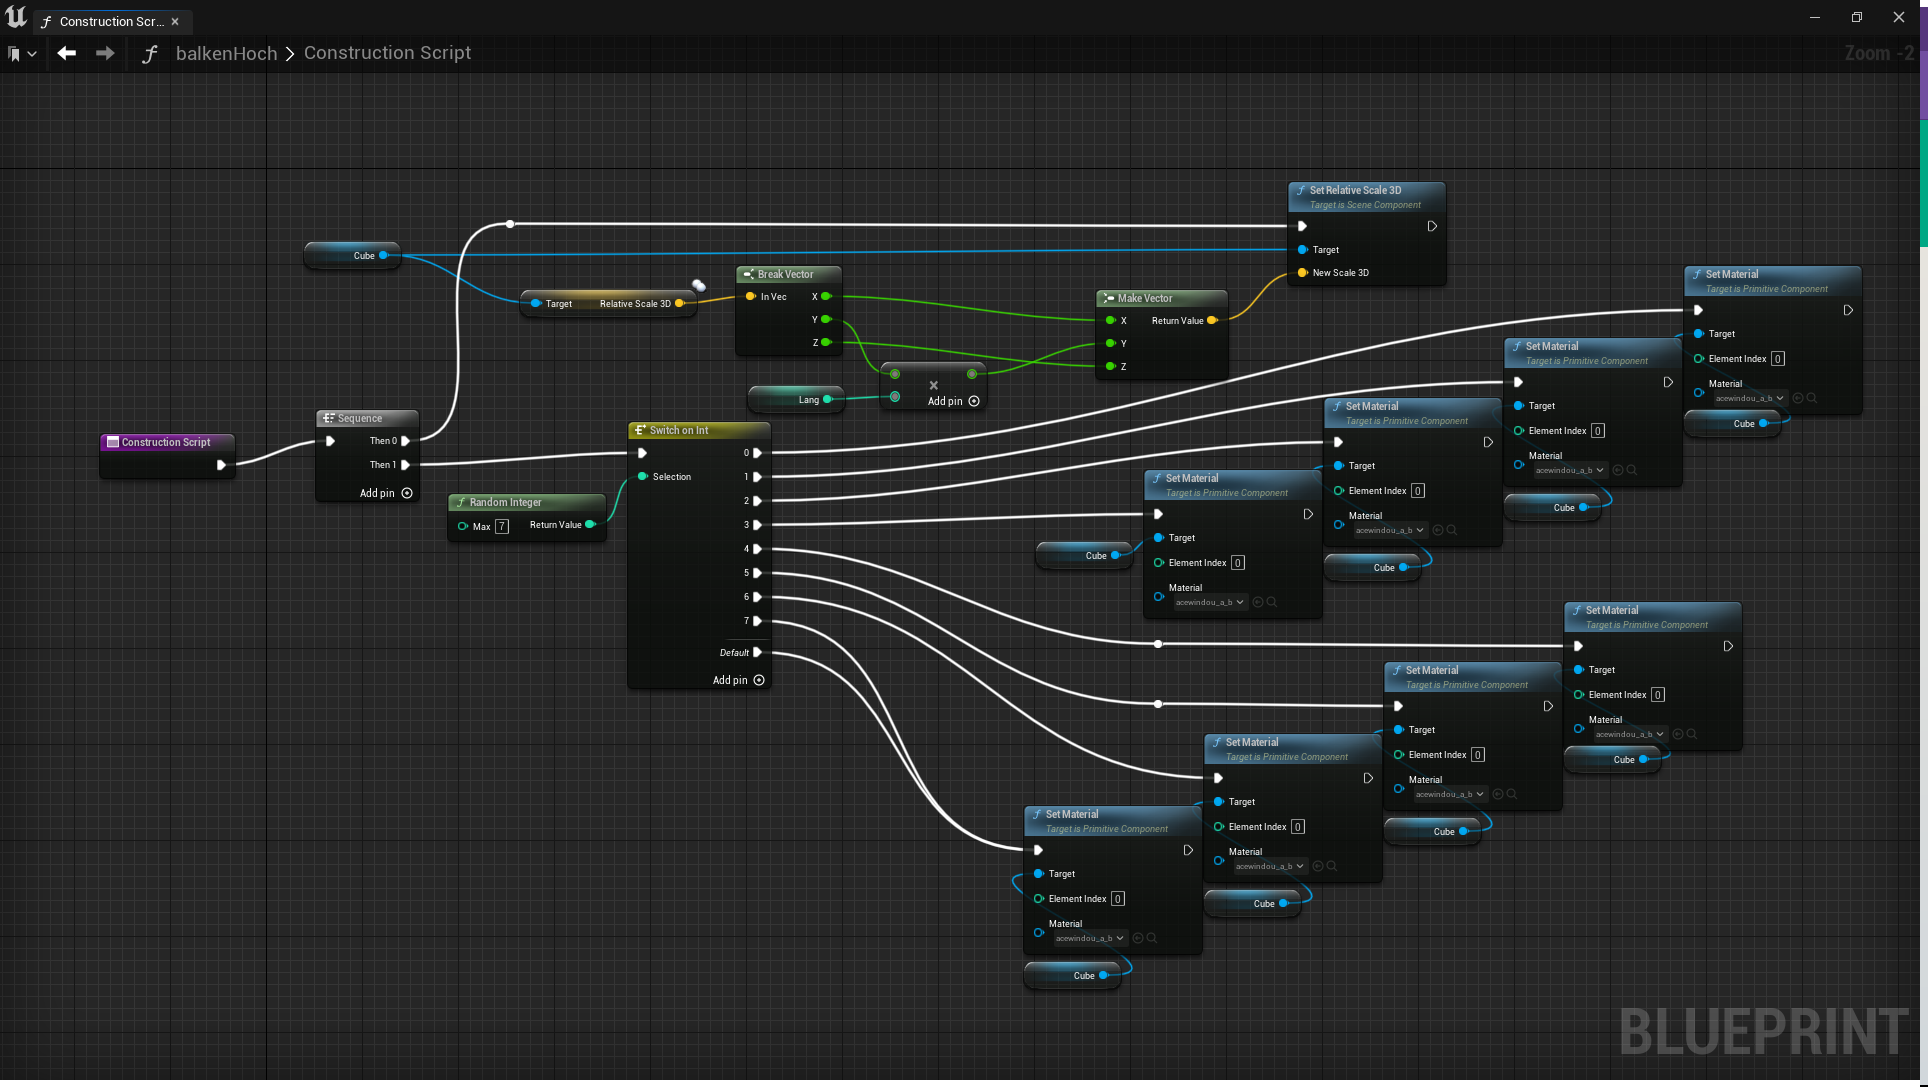
\includegraphics[width=14cm]{BilderFuerBA/balkenHochBP.png}
	\caption{UE5 Blueprint: Balken Hoch Construction Script}
	\label{UE5balkenHochBP}
\end{figure}
\section {Meilenstein: Nebenfiguren}
Beim dritten Meilenstein Nebenfiguren möchte ich gerne beschreiben, wie ich meine Nebenfiguren, kurz NPCs, erstellt habe. Ähnlich wie beim Erstellen der Hauptfigur habe ich durch Chat GPT mir verschiedene NPCs beschrieben lassen. Zu dieser Beschreibung gehörte Alter, Geschlecht, Beruf unnd charakterliche Eigenschaften.
\\
Mit diesen Beschreibungen habe ich mir einen Prompt mit hilfe der Midjourney-Formel überlegt und Midjourney hat mir Conceptgraphiken erzeugt. Nach mehreren Versuchen habe ich zwei Conzeptgraphiken bekommen die ich für PIFuHD verwenden kann.
\\
Nach dem ich PIFuHD die beiden Conzeptgraphiken übergebe, bekomme ich wie bei der Hauptfigur die 3D-Modelle der NPCs. In Blender habe ich den Polycount reduziert, die 3D-Modelle Texturiert und stark verformete Stellen nachgebessert.
\\
Für den Prototyp exportiere ich die NPCs ohne Sceleton Mesh sls FBX in Blender. Da die NPCs keine Spring oder laufanimation benötigen, sonder nur in der Spielwelt platziert werden um mit dem Hauptcharakter zu reden, benötigen die NPCs kein Skeleton Mesh.
\\
Nach diesen Arbeitsschritten kann ich die NPCs in die Unreal Engine 5 importieren und verteilen.
\begin{comment}
	%todo das ins fazit
	Dadurch das die NPC keine Sceleton Mesh besitzen ist auch gut zu erkennen, das die NPCs keine großen verformungen aufweisen wie die Hauptfigur. Die Verformung tritt z. B. in bereich der Hüfte sehr stark auf aufgrund der unterschiedlich gewichtete Zuweisung der Vertices zu den einzelnen Bones des Sceleton Mesh.
\end{comment}

%\\\\\\\\\\\\\\\\\\\\\\\\\\\\\\\\\\\\\\\\\\\\\\\\\\\\ Dialogsystem\\\\\\\\\\\\\\\\\\\\\\\
%\\\\\\\\\\\\\\\\\\\\\\\\\\\\\\\\\\\\\\\\\\\\\\\\\\\\ Dialogsystem\\\\\\\\\\\\\\\\\\\\\\\
%\\\\\\\\\\\\\\\\\\\\\\\\\\\\\\\\\\\\\\\\\\\\\\\\\\\\ Dialogsystem\\\\\\\\\\\\\\\\\\\\\\\
\section {Meilenstein: Dialogsystem}
Um ein Dialogsystem in der Unreal Enginge 5 zu entwickeln habe ich mehrere Ansätze gebraucht.

\subsection{Ansatz 1 mit ChatGPT}
Ich fordere ChatGPT dazu auf mir ein Dialogsystem zu entwickeln damit mein Hauptcharakter mit den NPCs aus meinem Prototyp sich unterhalten können.
\\
Ich habe versucht die Schritte umzusetzen die ChatGPT mir vorgegeben hat. Das Ergbenis dieser Anleitung die mir ChatGPT gezeigt hat, hat zu keinem Dialog meiner Charaktere geführt.
\\
Was ich zusätlich probiert habe ist ein Dialogsystem mit Hilfe von ChatGPT zu konzeptionieren.
\\
Dieses Konzept soll mehrere Dialogversionen erschaffen, und einfluss auf den Gesprächsverlauf ausüben.
\\
Eine Inspiration ist für mich die Sincefiction Spielereihe Mass Effect. In dieser Spielreihe is es möglich, durch Gespräche mit den NPCs verschieden verläufe zu erleben.
\\
Mein ziel ist es mit Hilfe von ChatGPT ein ähnliches einfache Dialoge zu kreiren, was nicht g hat.

\subsection{Ansatz 2 Rechersche mit Suchmaschienen im Internet}
Mit der Suchmaschiene Google bin ich auf ein Video auf Youtube gestoßen, was mir erklärt hat wie ich ein Dialogsystem in Unreal Engine 5 erstellt wird.
\\
ChatGPT hat mir im gegensatz zu dem Youtube-Video nicht mitgeteilt das es eine möglichkeit gibt zwischen Blueprint-Klassen zu Komunizieren, und diese geschieht über Interfaces.
\\
Zu dem beschriebenen Dialogsystem habe ich zusätzlich ein Dilay in der Länge von dem Soundfile hinzugefügt und ein Bool, der auf false steht, falls eine Interaktion gerade nicht möglich sein sollte.
\\
Dieser Bool verhindert, wenn ein Charakter gerade noch redet, ein weiteres Gespräch anfängt. Zusaätlich verhindert der Bool, dass keine Dialoge schnell hintereinander gestartet werden und die Charaktere aussprechen lassen.

%\\\\\\\\\\\\\\\\\\\\\\\\\\\\\\\\\\\\\\\\\\\\\\\\\\\\ Sprachausgabe\\\\\\\\\\\\\\\\\\\\\\\
%\\\\\\\\\\\\\\\\\\\\\\\\\\\\\\\\\\\\\\\\\\\\\\\\\\\\ Sprachausgabe\\\\\\\\\\\\\\\\\\\\\\\
%\\\\\\\\\\\\\\\\\\\\\\\\\\\\\\\\\\\\\\\\\\\\\\\\\\\\ Sprachausgabe\\\\\\\\\\\\\\\\\\\\\\\
\section {Meilenstein: Sprachausgabe}
Nachdem ich das Dialogsystem erstellt und implementiert habe, fehlt nur noch der Inhalt, was die Charaktere miteinander reden. Dazu brauche ich Aufnahmen von Stimmen. Kurz, Martin Luther sowie die beiden NPCs Anna und Johan, brauchen Synchronstimmen.
\\
Für das erzeugen der drei Synchronstimmen habe ich mit zwei weiteren KI-Systeme experimentiert, und möchte mein Vorgehen und das Ergebnis in diesem Kapitel präsentieren.
\\
Voice AI ist ein KI-System, die Stimmen verändern kann. Zum Beispiel kann man seine Stimme so manipulieren, das sie wie die von Kanye West oder dem amtierende US-Präsident Joe Biden klingt.
\\
Adobe Enhanced ist ein KI-System, das deine gesprochene Stimme so klingen lässt, dass sie in einem hochwertigen Tonstudio aufgenommen wird.
\\
Zu diesen beiden KI-Systemen, benutze ich mein neun Jahre altes Logitech G35 Headset um meine Stimme aufzunehmen.
\begin{comment}
	\\
	Durch die Kombination von Adobe Enhance Speech und Voice AI habe ich qualitativ hochwertige Sprach Dateien erzeugen können, die sonst ein hochwertiges Tonequipment und gute Dämmung in meinem Büro erzeugt hätten.
	\\
\end{comment}
Um die Stimmen für die NPCs zu erzeugen, habe ich drei verschiedene Experimente durchgeführt.
\\
\begin{itemize}
	
	\item Erst Adobe Enhance Speache dann Voice AI
	Als erstes wurde der Klang meiner stimme mit Audacity und meinem Logitech G35 Headset aufgenommen.
	\item Erst Voice Ai dann Adobe Enhance Speech
	\item Erst Adobe Enhance Speech dann Voice AI dann wieder Adobe Enhance Speech
\end{itemize} 
\begin{comment}
	Experiment eins, erst Voice I gegeben und dann Adobe Anshan Speech. 		 Oder? Erst Adobe, Assange Speech und dann Voice AI.  Ich habe noch eine dritte.
	\\
	
	Variante ausprobiert, und zwar eine Art Sandwich Methode, indem ich meine Sounddatei, die ich mit Audacity aufgenommen habe, erst Adobe 1. Hand speech. Dann Voice I und dann wieder Adobe A Speech gegeben habe, um so eine Art zweifache Reinigung. Der Sprache oder der Sprachausgabe zu erhalten.     Mein persönliches bestes Ergebnis, was auch Zeittechnisch am. Sparsamsten war.  Ist erst.  Athan Speech zu benutzen und dann Voice I. Die dritte Version ist auch ok, aber es kann sein, dass danach sich die Stimme noch etwas künstlicher, Blecherner anhört.   Generell ist die Sprachausgabe sehr.  Gut.
	\\
	Und professionell anwendbar für mein Prototyp ist das eine Qualität, die ich früher nicht erreicht hatte können außer mit großen Aufwand und Kosten verbunden wie ZB das Kaufen eines 200€, Mikrofons und sehr guter Dämmung in meinem Aufnahmeraum. Ich habe die Aufnahmen bei einem sonnigen Tag während. Traktoren im Hintergrund arbeiten. Ich habe in meinem Arbeitszimmer. Ein Fenster aufgehabt. Das offenbar zu einem Bauernhof in meiner Nachbarschaft. Man kann Traktoren hören, man kann meine Frau hören, im Hintergrund, die in der Wohnung mit den Kindern sich beschäftigen und anhand Speech hat das alles herausgefiltert. Und ein gewisses Grundrauschen befindet sich auch nicht mehr und der Sound-Datei.
	\\
	Die Meilensteine.  Die ich hier in meiner Bachelor thesis beschreibe.  Sind nicht chronologisch sortiert, sondern nur logisch.  Ich habe das Dialogsystem und die Sprachausgabe gleichzeitig entwickelt und.  Implementiert.  Die Sprachausgabe, die ich hiermit mit Voice I und Adobe anhand Speech. Geschaffen habe, habe ich nun in das.  Dialogsystem was sich in dem vorigen Kapitel beschrieben habe. Implementiert. Ich habe die Sprachausgabe in das Array getan.		 In der andere Engine 5.
	
	\section{Erstellung von Musik und Klängen}
	\section{Erstellung von Animationen}
	\section{Entwicklung der Spiellogik}
\end{comment}
\chapter{Ergebnisse und Diskussion}

\section{Vorstellung des fertigen Videospiels}
 
\section{Diskussion der Ergebnisse und Einschätzung des Erfolgs des KI-Einsatzes}

\subsection{Einsatz von MonsterMash}
Monster Mash ist ein KI-System, mit dem man Monster erstellen kann. Wenn man sich realitätsnahe Ergebnisse wünscht, wird man mit Monster Mash auf sehr große Herausforderungen treffen.
\\
Monster sind Fantasiewesen, und niemand kann genau beschreiben, wie ein Monster aussieht. Bei der Darstellung von Menschen oder Gebäuden sieht das anders aus. Für mein Adventure-Game, mit einem historischen Hintergrund, ist MonsterMash nicht zu empfehlen.
\\
Anders würde es in einem Fantasy-Szenario aussehen, wo undefinierte Gestalten dem Spieler begegnen sollen.

\subsection{Einsatz von PFuHD}
PIFuHD ist eine KI-System was darauf trainiert ist, Digitalfotos von Personen in ein 3D-Modell umzuwandeln. PIFuHD kann man auf Google-Collab einrichten und lauffähig machen.
\\
Für das erstellen von 3D-Modellen wurde PIFuHD ist in der kostenlosen Demo-Version verwendet.
\\
Die Kompatibilität zwischen Midjourney und PIFuHD ist möglich. Die Resultate sind zum teil Artefakt belastet, die besonders in Bereichen der Hände, Füße und Kleidung auftreten.
\\
Durch Midjourney konnte ich Bilder von Martin Luther erzeugen, die als Konzeptgrafiken dienten. Diese Konzeptgrafiken habe ich PIFuHD als eingabe gegeben, und hat mir daraus folgende 3D-Modelle von Personen ausgegeben, die im Prototyp als Hauptfigur und NPCs verwendet wurden.


\section{Kritische Reflexion des Entwicklungsprozesses und Ausblick auf mögliche zukünftige Entwicklungen}
\chapter{Allgemeine Probleme mit KI und KI-Systeme}

Ich möchte an dieser Stelle auf eine Auswahl gesellschaftliche Punkte eingehen, die mich während meiner Arbeit mit und über KI-Systeme begegnet sind und mich als Ein-Mann-Videospielentwickler begleitet haben.


\section{KI-Systeme und ihrer Monatarisierung}
%steam verbietet verkauf von ki-asset speiele

\section{KI-Systeme und ursachen auf andere Berufe
}%entwickler in china entlässt concet artist um selber mit ki-systemen wie midjourney zu arbeiten

\section{Ki-Systeme und der Biologischer Fussabdruck}
%ki-systeme verbrauchen viel strom um sie zu trainieren

\section{KI-Systeme aund die auswirkung als Entwickler}
%wahrscheinlich persönlich was ich immer gedacht habe immer ki immer ki und weniger selber nachdenken.. man sollte auch vertrauen auf seine fähigkeiten haben, oder auf seine menschliche gesellschaft hilfe suchen. es icht nicht schlimm ein musiker nach musik zu fragen, und zu bezahlen.

\section{Dritte-Welt länder vs. Erste-Welt länder}
%ki-systeme werden offt in schwellenländer trainiert für ein hungerlohn

\section{Firmeninteressen}
%die entwickler solcher ki-systeme haben eigene interessen wie Politik china und tiktok.. china klavier usa gefährliche chellenges

\section{Geistiges Eigentum}
%zum beispiel JR-Tolkin un die US-Schriftsteller verband verkagen OpenAI da sie Texte zum Trainieren benutzen ohne zustimmung, genau so wie berühmte Digital Artist in steal von  Studio gibli und kuvshinov digital artist die über jahrzehnte ihren stil entwicklet haben

\chapter{Fazit}

Fragestellung: Welche Möglichkeiten bieten KI-Systeme einem Ein-Mann-Videospieler bei der Entwicklung eines Videospiels?  

In dieser Arbeit wurde der Frage nachgegangen, welche Möglichkeiten KI-Systeme einem Ein-Mann-Videospieler bei der Entwicklung eines Videospiels bieten. 

Anhand der Entwicklung meines Prototypen, habe ich herausgearbeitet, dass ….


KI-Systeme laden zum Experimentieren ein. Als Ein-Mann-Videospieler ist es möglich, einen Plot für Videospiele in Minuten zu schreiben, wofür ich Wochen benötigen würde und das nur durch einen einfachen Prompt für ChatGPT.
\\
Ich kann Konzeptgrafiken, UX-Elemente, Texturen in Hülle und Fülle mit Midjourney generieren, ohne nur einen Stift oder Grafiktablett in die Hand zu nehmen.
\\
Als Legastheniker und untalentierter Maler und Zeichner bieten mir KI-Systeme noch nie da gewesene Möglichkeiten, mich kreativ auszuleben.
\\
Die in Kapitel 5 verwendeten KI-Systeme sind nur ein Beispiel, mit denen ich gute und sinnvolle Ergebnisse für meinen Prototyp erstellt habe. Ich habe mich mit vielen weiteren KI-Systemen beschäftigt und diese ausprobiert, die aber in der Entwicklung meines Prototypes keinen Einfluss hatten.
\\
KI-Systeme wie zum Beispiel MonsterMash, mit dem man mit einem Hintergrundbild und einer Zeichnung mit der Maus ein einfaches 3D-Modell erzeugen kann. Dieses 3D-Modell kann man mit Hilfe von bewegbaren Punkten animieren.
\\
Ich habe die Photoshop-KI von Adobe ausprobiert. Mit diesem KI-System konnte ich zum Beispiel die Texturen, die ich für mein einfaches Haus von Midjourney bekomme, so bearbeiten, dass aus einer Tür ein Fenster wird.
\\
Ich wollte mit einem KI-System namens Kaedim arbeiten, da sie einer der wenigen KI-Systemen die fähigkeit besaß, aus Bildern 3D-Modelle zu erzeugen. Der Preis von circa 15€ pro Prompt hat mich abgeschreckt. Hinzu kam das Kaedim eine sehr lange bearbeitungszeit benötigt hätte, von ca 20 Minuten war die Rede, was ich in diesem Moment sehr Merkwürdig fand.
Durch ein Blick in der Dokumentation, wurde Kaedim so beschrieben, das es eine Mischung aus einem Trainierten KI-System und 3D-Artist ist, von dem ich das Ergebnis bekommen würde.
Da ich mich als Ein-Mann-Videospielerentwickler sehe, habe ich mich dazu entschieden, dieses KI-System zu verwenden, da ich erstmal keinen anderen Menschen an meinem Prototyp arbeiten lassen möchte.
\\
Ich habe mich auch auf Soundful Music und AIVA angemeldet und versucht in Richtung Music zu forschen und Experimentieren, aber meine Zeit das leider nicht zugelassen.
\\
Musik finde ich ein Spannendes gebiet, und es gibt KI-Systeme die sich in diesem Thema sich bewegen. Leider hatte ich keine zeit im Rahmen meiner Bachelorthesis mich in dieser Richtung intensiv zu experimentieren.
\\
Während meiner Projektphase hatte ich immerwieder das gefühl, das das Wort KI und AI oft als Marketing buzzwort benutz haben um sich vom Markt abzuheben.
\\
KI-Systeme zu erforschen und erfahren, kann sehr viel zeit in Anspruch nehmen. Mit jedem Neuen System muss man üben. Jedes KI-System hat grenzen die die Erwartungen oder Anforderung eines Ein-Mann-Videospieleentwickler entsprechen.
\\
Ich möchte in diesem Fazit ein wenig bildlich werden.
\\
Wenn ein Videospiel Prototyp ein dreistöckiges Haus wäre:
Das Fundament, der Keller und alle Leitungen wie Wasser, Strom und Gas ist die Unreal Engine 5.
Der Erste- sowie die Hälfte des Zweiten-Stocks, der größte Teile der Außen- und Innenfassade, können Ergebnisse von KI-Systemen sein.
Der Rest hängt von dem Ein-Mann-Videospielentwickler und seinen Fähigkeiten ab um ein schlüsselfertiges Haus zu bauen.
\\
Mein Prototyp hat eine erkennbare Form, ist aber noch weit davon entfernt um Potenzielle Geldgeber, wie die Deutsche Gameförderung, zu überzeugen um mich als Ein-Mann-Videospielentwickler Geld zu bekommen um aus meinem Prototyp ein Fertiges, marktreifes Spiel zu erschaffen.
\\
Mein Ziel war es, Inhalte für mein Prototyp mit Hilfe von KI-Systemen für die Unreal Engine 5 zu erschaffen, und ich bin So


\section{Zusammenfassung der Ergebnisse}
\section{Implikationen für die Praxis}
\section{Limitationen der Studie}

%\pagenumbering{Roman}
\pagenumbering{Roman}
\setcounter{page}{5} % Seitenzahl zählt 
\chapter{Anhang} 
% Anstatt Abbildungen und Diagramme



\addpart{Abbildungsverzeichnis} %Erstellt Eintrag ins Literaturverzeichnis
%\adpart{}
\listoffigures
\listoftables
\chapter*{Code-Beispiele}

\bibliographystyle{apalike-german}
\bibliography{ref}

\chapter*{Weitere Materialien}
\end{document}
